\section[Information on Discursive Sophistication Components]{Detailed Information on Open-Ended Responses and Discursive Sophistication Components}\label{app:oeinfo}
%\renewcommand\thefigure{A.\arabic{figure}}
%\renewcommand\thetable{A.\arabic{table}}
%\setcounter{figure}{0}
%\setcounter{table}{0}


\subsection{Distribution of Word Counts in Open-Ended Responses}

\begin{figure*}[h]
    \centering
    \begin{subfigure}[t]{0.49\textwidth}
        \centering
        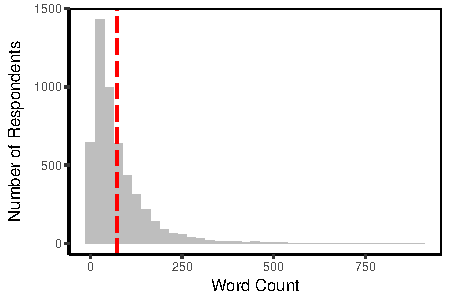
\includegraphics{/data/Dropbox/Uni/Projects/2016/knowledge/fig/anes2012_wc.pdf}
        \caption{2012 ANES}
    \end{subfigure}%
	\begin{subfigure}[t]{0.49\textwidth}
        \centering
        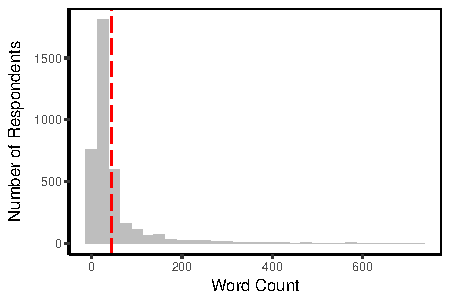
\includegraphics{/data/Dropbox/Uni/Projects/2016/knowledge/fig/anes2016_wc.pdf}
        \caption{2016 ANES}
    \end{subfigure}%
    
    \begin{subfigure}[t]{0.49\textwidth}
        \centering
        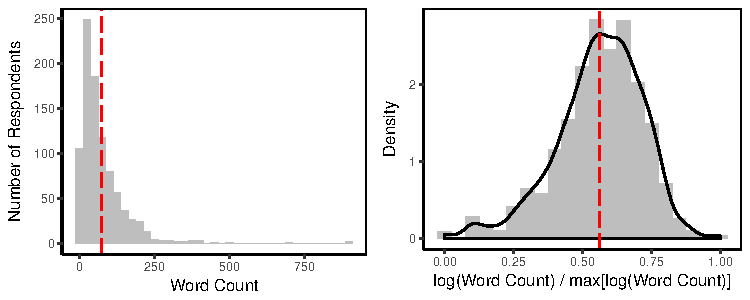
\includegraphics{/data/Dropbox/Uni/Projects/2016/knowledge/fig/yg_wc.pdf}
        \caption{2015 YouGov}
    \end{subfigure}
    \begin{subfigure}[t]{0.49\textwidth}
         \centering
         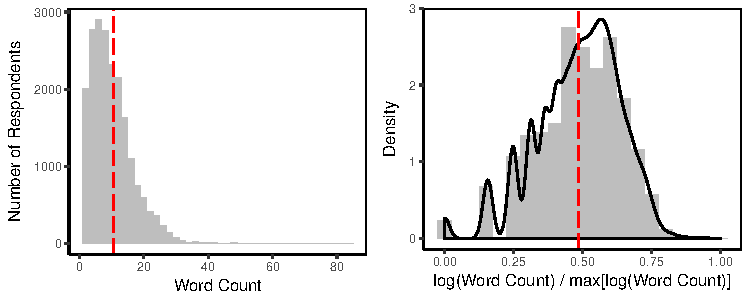
\includegraphics{/data/Dropbox/Uni/Projects/2016/knowledge/fig/swiss_wc.pdf}
         \caption{Swiss Survey}
    \end{subfigure}
    \caption[Histograms of total word count in open-ended responses]{Histograms of total word count in the collection of open-ended responses for each individual. The dashed red lines indicate the average response lengths in each survey.}\label{fig:wc}
\end{figure*}


\clearpage
\subsection{Overview of Topic Proportions}

\begin{figure}[h]\centering
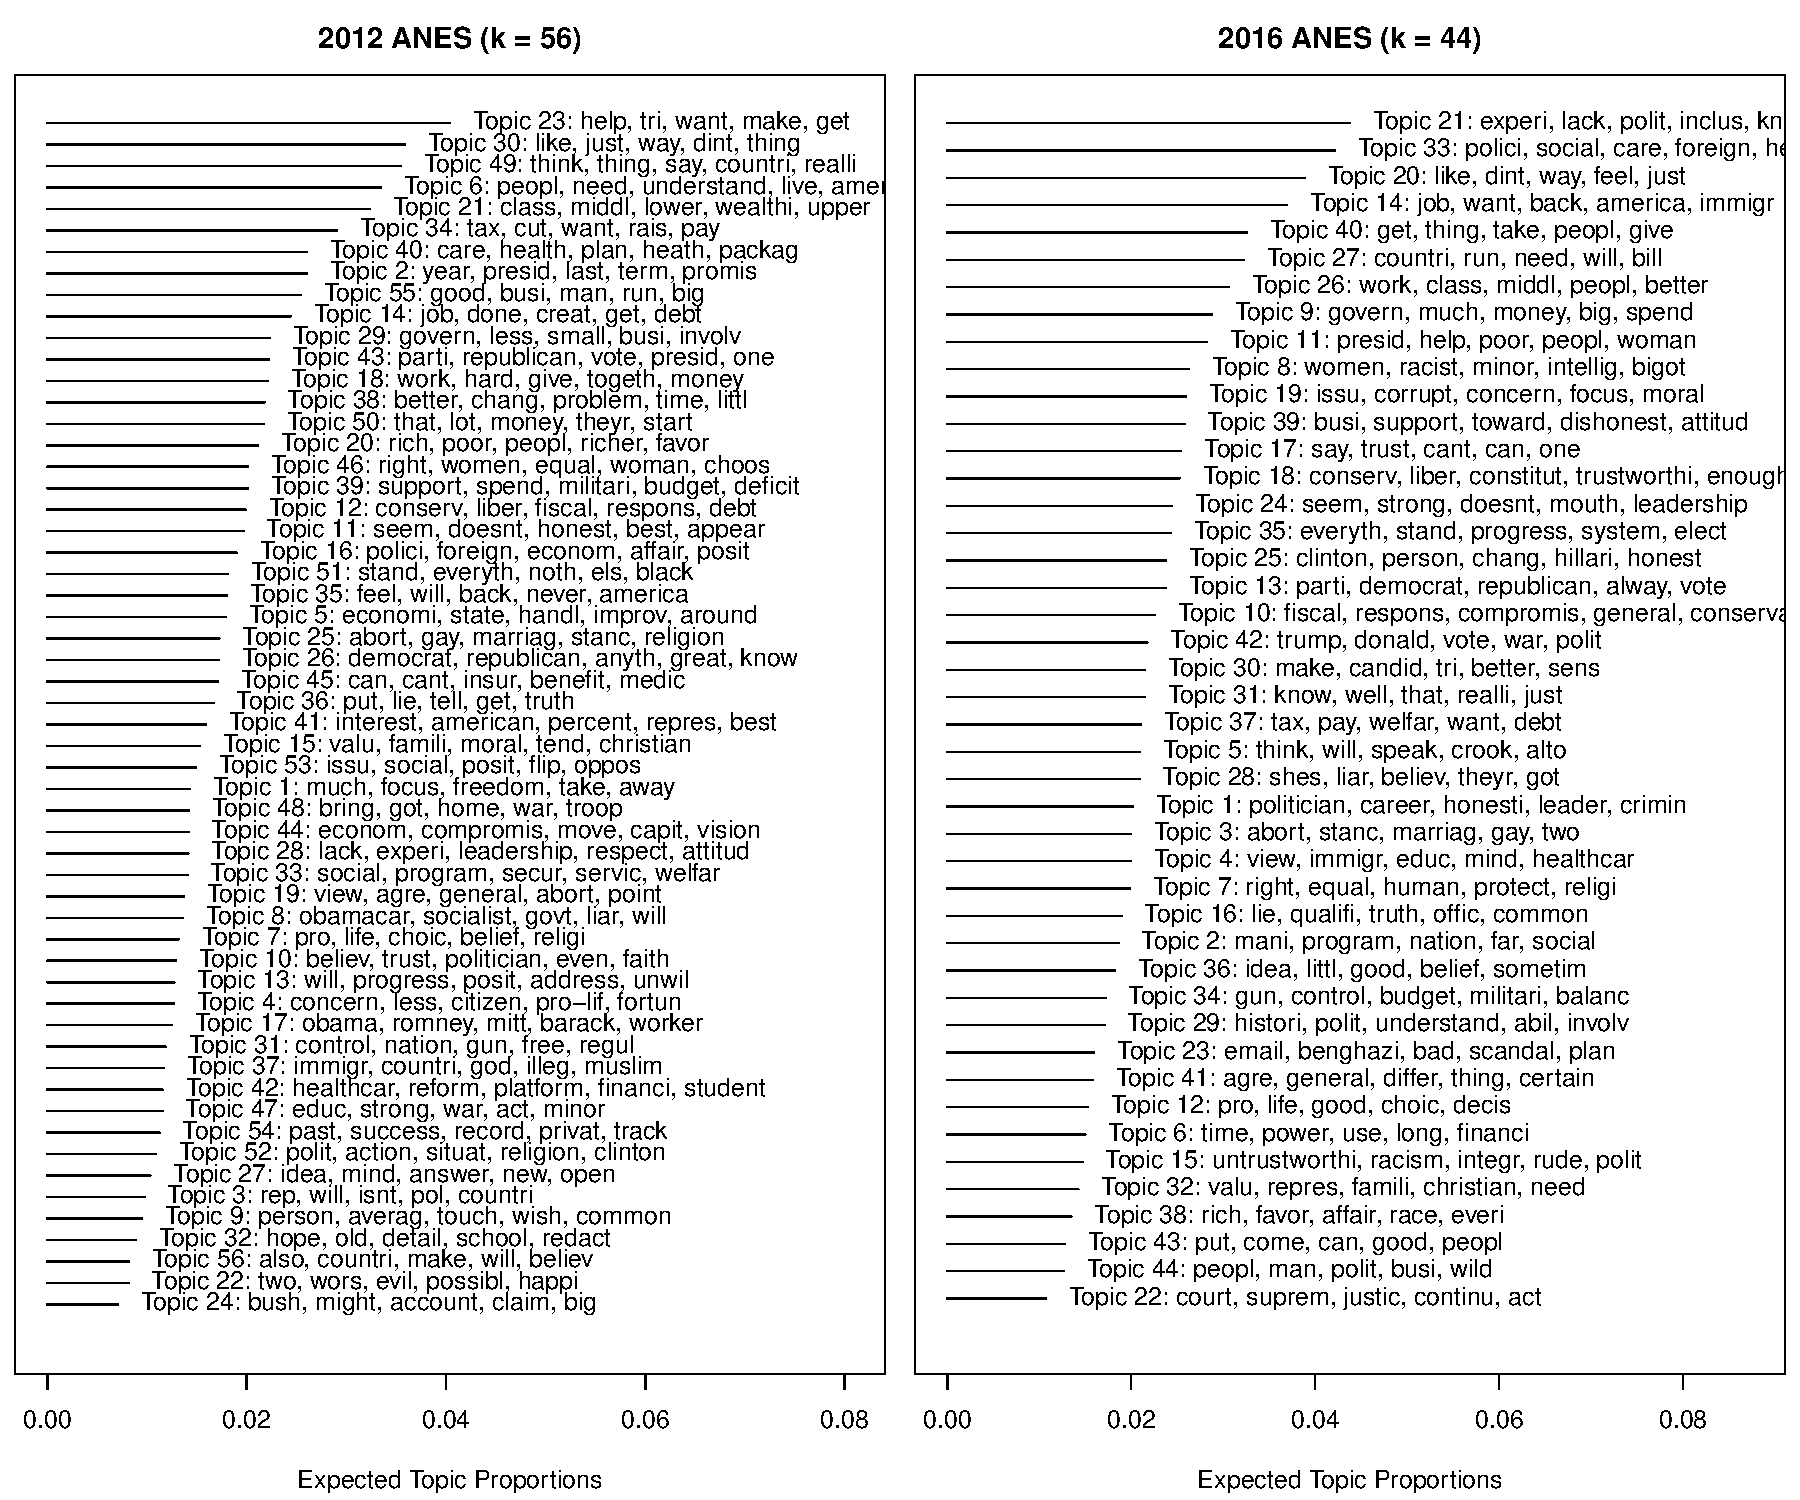
\includegraphics[width=\textwidth]{/data/Dropbox/Uni/Projects/2016/knowledge/fig/anes_stm_prop.pdf}
\caption[Estimated topic proportions in the 2012 and 2016 ANES based on the structural topic model]{Estimated topic proportions in the 2012 and 2016 ANES based on the structural topic model. See Appendix~\ref{app:topicmodel} for details on the model specification.}\label{fig:anes_stm_prop}
\end{figure}

\begin{figure}[h]\centering
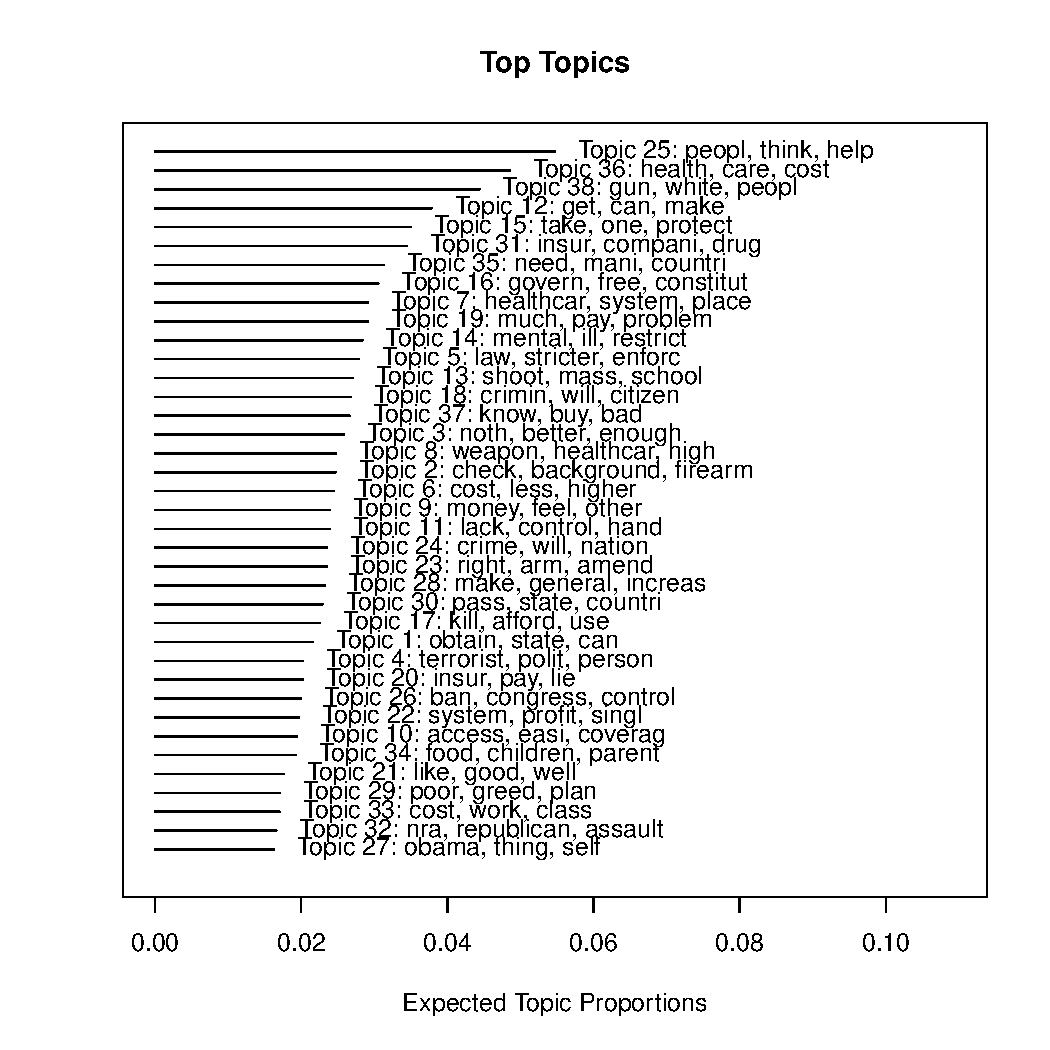
\includegraphics[width=.5\textwidth]{/data/Dropbox/Uni/Projects/2016/knowledge/fig/yg_stm_prop.pdf}
\caption[Estimated topic proportions in the 2015 YouGov survey based on the structural topic model]{Estimated topic proportions in the 2015 YouGov survey based on the structural topic model. See Appendix~\ref{app:topicmodel} for details on the model specification.}\label{fig:yg_stm_prop}
\end{figure}

\begin{figure}[h]\centering
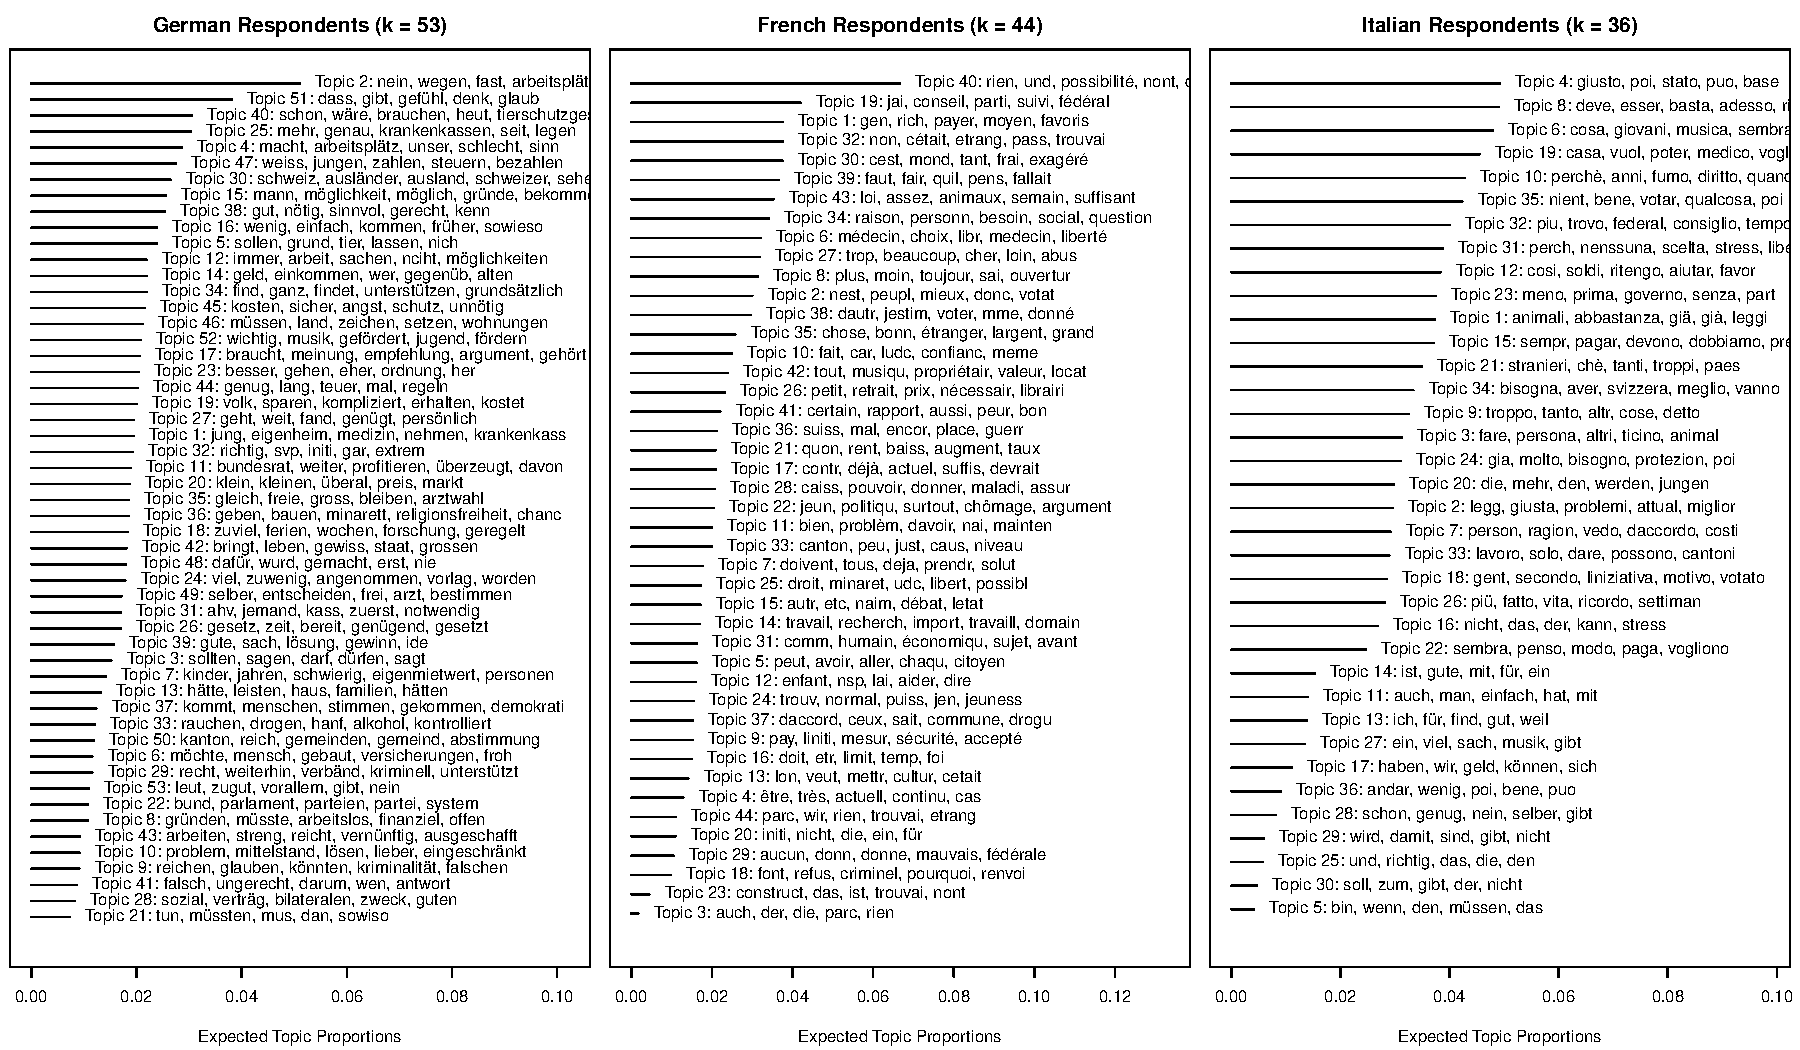
\includegraphics[width=\textwidth]{/data/Dropbox/Uni/Projects/2016/knowledge/fig/swiss_stm_prop.pdf}
\caption[Estimated topic proportions in the Swiss survey based on the structural topic model]{Estimated topic proportions in the Swiss survey based on the structural topic model. See Appendix~\ref{app:topicmodel} for details on the model specification.}\label{fig:swiss_stm_prop}
\end{figure}


\clearpage
\subsection{Discursive Sophistication Components}
\begin{figure*}[h]
    \centering
    \begin{subfigure}[h]{0.4\textwidth}
        \centering
        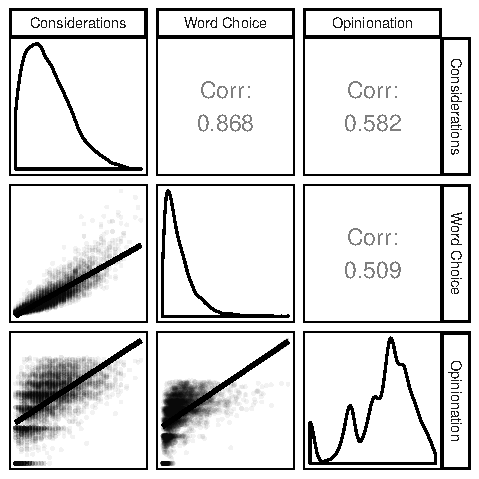
\includegraphics{/data/Dropbox/Uni/Projects/2016/knowledge/fig/anes2012_corplot_components.pdf}
        \caption{2012 ANES}
    \end{subfigure}%
    \begin{subfigure}[h]{0.4\textwidth}
         \centering
         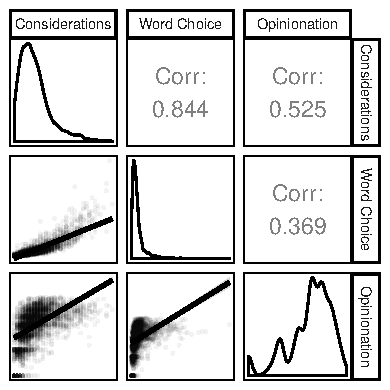
\includegraphics{/data/Dropbox/Uni/Projects/2016/knowledge/fig/anes2016_corplot_components.pdf}
         \caption{2016 ANES}
    \end{subfigure}%
    
    \begin{subfigure}[h]{0.4\textwidth}
        \centering
        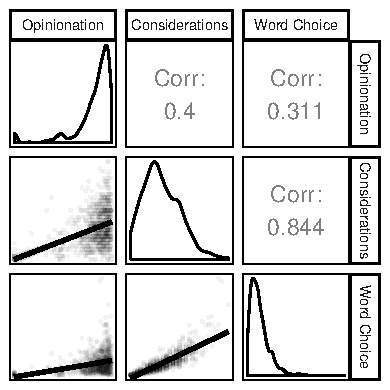
\includegraphics{/data/Dropbox/Uni/Projects/2016/knowledge/fig/yg_corplot_components.pdf}
        \caption{2015 YouGov}
    \end{subfigure}%
    \begin{subfigure}[h]{0.4\textwidth}
         \centering
         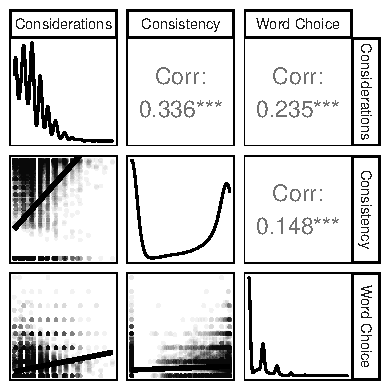
\includegraphics{/data/Dropbox/Uni/Projects/2016/knowledge/fig/swiss_corplot_components.pdf}
         \caption{Swiss Survey}
    \end{subfigure}
    \caption[Correlation matrix of individual components of discursive sophistication.]{Correlation matrix of individual components of discursive sophistication. The plots on the diagonal display univariate densities for each component. The panels in the lower triangular display the scatter plot of two measures as well as a linear fit. %The upper triangular displays the correlation coefficient.
     }\label{fig:components}
\end{figure*}



\clearpage
\section{Pre-Processing and Topic Model Specification}\label{app:topicmodel}
%\renewcommand\thefigure{B.\arabic{figure}}
%\renewcommand\thetable{B.\arabic{table}}
%\setcounter{figure}{0}
%\setcounter{table}{0}

\subsection{PreText Analysis}
Two components of discursive sophistication (\textit{considerations} and \textit{word choice}) rely on quantities extracted from structural topic models \citep{roberts2014structural}. As with any other text-as-data approach, a necessary first step before estimating the topic model is to pre-process the raw text and convert it into a document term matrix \citep[DTM, see for example][]{manning2008introduction}. Common pre-processing procedures include stemming and lowercasing, as well as the removal of numbers, punctuation, stopwords, and infrequent terms. However, topic models and other unsupervised learning techniques can be sensitive to these pre-processing choices \citep[c.f.,][]{denny2018text}. To address this issue, \citet{denny2018text} recommend that researchers compare DTMs under all possible pre-processing regimes. The authors propose \textit{preText scores} as a measure to quantify the extent to which varying pre-processing regimes may yield unusual results compared to a baseline without any pre-processing.

\begin{figure}[h]
\centering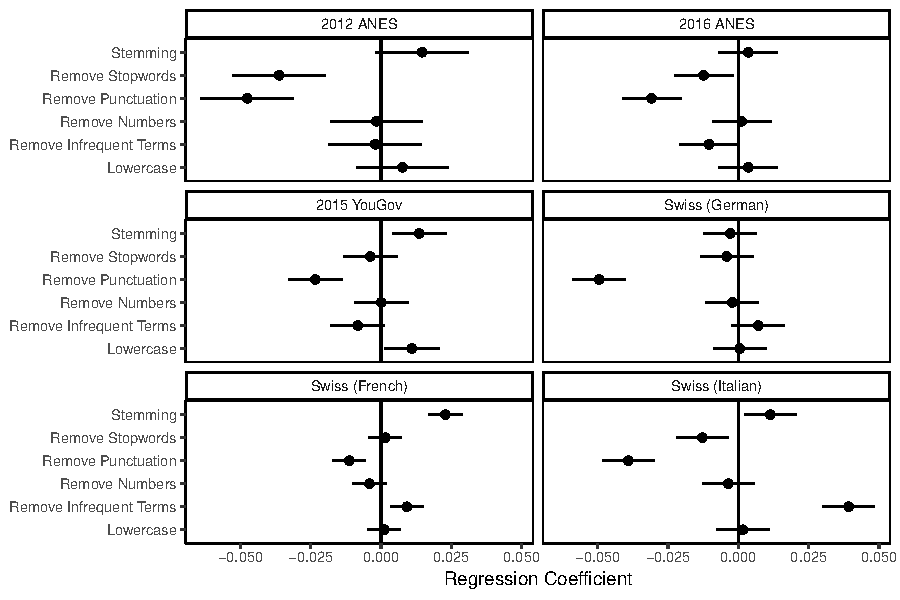
\includegraphics{/data/Dropbox/Uni/Projects/2016/knowledge/fig/pretext.pdf}
    \caption[PreText analysis of pre-processing decisions of open-ended responses across all datasets]{PreText analysis of pre-processing decisions of open-ended responses across all datasets. Regression coefficients display the effects of each of the six pre-processing choices on the resulting preText score.}\label{fig:pretext}
\end{figure}


\subsection{Robustness Checks for Varying Model Specifications}

Following the procedure outlined in \citet{denny2018text}, Figure~\ref{fig:pretext} displays the results of a linear model regressing preText scores resulting from all possible pre-processing regimes on each individual step for a random subset of 500 open-ended responses in each of the studies included in the analyses. Significant coefficients indicate that the topic model results my be sensitive to the respective pre-processing step. As such, removing stopwords and punctuation, as well as removing infrequent terms (at least in the 2016 ANES) might be problematic. \citet{denny2018text}, however, emphasize that the most important consideration in choosing pre-processing steps are theoretical. Given that the purpose of the topic model is to extract considerations related to political preferences, there are strong theoretical reasons to remove stopwords and punctuation from open-ended responses as they do not contain any relevant content. Furthermore, I apply lowercasing and stemming of terms to reduce resulting document term matrix to a computationally more manageable size and since these pre-processing steps should not be influential according to the preText analysis.

It is less obvious from a theoretical perspective whether to remove infrequent terms from open-ended responses, although it is preferred in order to make the estimation of the discursive sophistication components computationally efficient. Since the preText analysis for the 2016 ANES suggests that this pre-processing step might be influential, I compare discursive sophistication for both alternative regimes below \citep[c.f.,][]{denny2018text}. Before turning to this sensitivity check, however, I consider another crucial modeling choice when working with topic models: determining the total number of topics $k$ to be estimated. For all analyses reported below, the number of topics was selected using the algorithm proposed by \citet{lee2014low} and implemented in the \texttt{stm} package in \textbf{R} \citep{roberts2014stm}.\footnote{I used measures for age, gender, education, party identification, as well as an interaction between education and party identification as covariates for topic prevalence. This variable selection---with the exception of including gender---is equivalent to the procedure model specification described in \citet{roberts2014structural}.} 

\begin{figure}[h]\centering
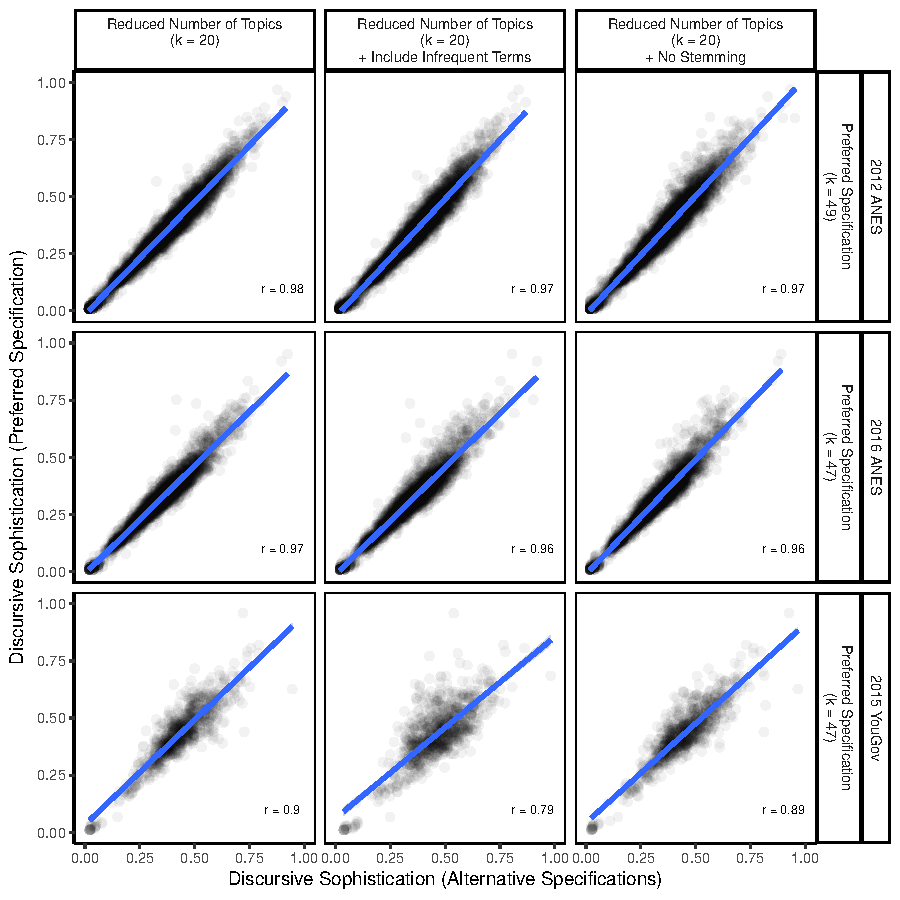
\includegraphics{/data/Dropbox/Uni/Projects/2016/knowledge/fig/pretext_robustness.pdf}
\caption[Robustness of discursive sophistication measure for different pre-processing choices and topic model specifications]{Robustness of discursive sophistication measure for different pre-processing choices and topic model specifications.}\label{fig:pretext_robustness}
\end{figure}

Figure~\ref{fig:pretext_robustness} examines whether the proposed measure of discursive sophistication is sensitive to the removal of infrequent terms as well as the chosen number of topics $k$. The y-axis depicts the preferred pre-processing regime including all steps discussed above while the x-axis plots results for alternative specifications. The panels on the left compare the preferred specification to discursive sophistication based on a reduced number of topics ($k=20$). The middle panels additionally include infrequent terms instead of removing them.\footnote{Calculating discursive sophistication with large numbers of topics while including infrequent terms is computationally prohibitive.} The panels on the right do not perform stemming as part of the pre-processing step. Across all panels, discursive sophistication scores are highly correlated and therefore insensitive to pre-processing choices and varying numbers of topics.

In summary, open-ended responses in the analyses reported in the main text are pre-processed by stemming and lowercasing, as well as the removing numbers, punctuation, stopwords, and infrequent terms (i.e., terms that appear in fewer than 10 responses).\footnote{Prior to applying these pre-processing steps, open-ended responses in the 2012 \& 2016 ANES as well as the 2015 YouGov survey are cleaned by correcting spelling errors using an implementation of the Aspell spell-checking algorithm (\url{www.aspell.net}).} While the results discussed in the manuscript are based on this preferred specification, the substantive results are robust for alternative pre-processing regimes or varying numbers of topics.


\clearpage
\section{Additional Information on Remaining Variables}\label{app:variables}
%\renewcommand\thefigure{C.\arabic{figure}}
%\renewcommand\thetable{C.\arabic{table}}
%\setcounter{figure}{0}
%\setcounter{table}{0}

\subsection{Item Selection and Recoding}

\paragraph{Conventional measures of political knowledge:}
\begin{itemize}
\item \textit{2012 ANES}: Additive index of correct responses to 5 knowledge items included in the pre-election wave (number of Presidential terms, size of budget deficit, length of Senate term, meaning of Medicare, federal government spending). `Don't know' responses are considered incorrect. Interviewer evaluations are based on the assessment of the respondent's general level of information about politics recorded at the end of the pre-election wave.
\item \textit{2016 ANES}: Additive index of correct responses to 4 knowledge items included in the pre-election wave (length of Senate term, federal government spending, majority in House, majority in Senate). `Don't know' responses are considered incorrect. Interviewer evaluations are based on the assessment of the respondent's general level of information about politics recorded at the end of the pre-election wave.
\item \textit{2015 YouGov Survey}: Additive index of correct responses to 8 knowledge items (Speaker of the House, meaning of TPP, Chair of Federal Reserve Board, current unemployment rate, Presidential veto override, meaning of Common Core, leading source of electricity in US, majority in Senate). `Don't know' responses are considered incorrect.
\end{itemize}

\paragraph{Dependent variables:}
\begin{itemize}
\item \textit{Turnout} (2012 \& 2016 ANES): Dichotomous indicator, based on post-election wave.
\item \textit{Non-conventional participation} (2012 \& 2016 ANES): Additive index of different forms of political engagement (participated in protest, signed petition, wore campaign button, wrote letter to public official).
\item \textit{Internal efficacy} (2012 \& 2016 ANES): Sum of two agree/disagree items (politics too complicated, good understanding of political issues [reversed]).
\item \textit{External efficacy} (2012 \& 2016 ANES): Sum of two agree/disagree items (public officials don't care, people have no say about what the government does).
\item \textit{Information retrieval (2015 YouGov Survey)}: Additive index of correct answers to 9 questions about the fictional disease described in the news article (symptoms: fatigue, headaches, diarrhea, joint pain, boils, warts, fever; virus spread; cure for the virus)
\item \textit{Candidate policy positions} (2012 \& 2016 ANES): Placement of Republican and Democratic Presidential candidates on 7-point scale (ideology, government spending, defense spending, insurance policy, job guarantee, aid to Blacks, environment vs jobs).
%\item \textit{Correct voting} (2012 \& 2016 ANES): Dichotomous indicator created according to the procedures described in \citet{lau1997voting,lau2008exploration} and \citet{sokhey2012social}. Correct votes are determined by party identification, overlap in issue positions (see above), and attachments to social groups that are aligned with each candidate. All components are weighted equally. Overlap in issue positions is conceptualized using directional voting scores \citep{rabinowitz1989directional}, where ``true'' candidate positions are determined by averaging perceived positions for highly knowledgeable respondents (scoring above median factual knowledge). Social groups (e.g., middle class, unions, tea party, etc.) are viewed as aligned with a candidate if group attachment differs significantly and in direction between highly knowledgeable (above median factual knowledge) supporters of each candidate (i.e., knowledgeable supporters of one group view them negatively on average while knowledgeable supporters of the other group view them positively on average).
\end{itemize}

\paragraph{Control variables:}
\begin{itemize}
\item \textit{Gender} (2012 \& 2016 ANES, 2015 YouGov Survey): Dichotomous indicator for female respondents.
\item \textit{Wordsum vocabulary scores}  (2012 \& 2016 ANES): Modified version of the GSS wordsum vocabulary test consisting of 10 terms.
\item \textit{Media exposure} (2012 \& 2016 ANES): Additive index of the frequency of weekly exposure to various political information sources such as newspapers or TV news (2012 ANES). In the 2016 ANES, it only consists of a single item measuring the number of days in the past week the respondent has spent watching/reading/listening news on any media.
\item \textit{Political discussion frequency} (2012 \& 2016 ANES): Self-reported count of days in the past week spent discussing politics with family or friends.
\item \textit{College education} (2012 \& 2016 ANES, 2015 YouGov Survey): Dichotomous indicator for Bachelor's degree or higher.
\item \textit{Family/Household income} (2012 \& 2016 ANES, 2015 YouGov Survey): Self-reported household income categories.
\item \textit{Age} (2012 \& 2016 ANES, 2015 YouGov Survey): Logged age in years.
\item \textit{Race} (2012 \& 2016 ANES, 2015 YouGov Survey): Dichotomous indicator for black non-Hispanic vs. others.
\item \textit{Church attendance} (2012 \& 2016 ANES, 2015 YouGov Survey): Six-category indicator of the frequency of church attendance. 
\item \textit{Survey Mode} (2012 \& 2016 ANES): Dichotomous indicator for face-to-face vs. online samples of the ANES surveys.
\item \textit{Personality characteristics} (2012 \& 2016 ANES): Measures of extraversion and being reserved, part of the Ten Item Personality Inventory (TIPI) measuring the ``Big Five'' personality traits.
\item \textit{Response length} (2012 \& 2016 ANES): Logged number of words in the collection of open-ended responses by each individual.
\end{itemize}


\clearpage
\subsection{Variable Distributions -- 2012 ANES}
\begin{figure}[h]\centering
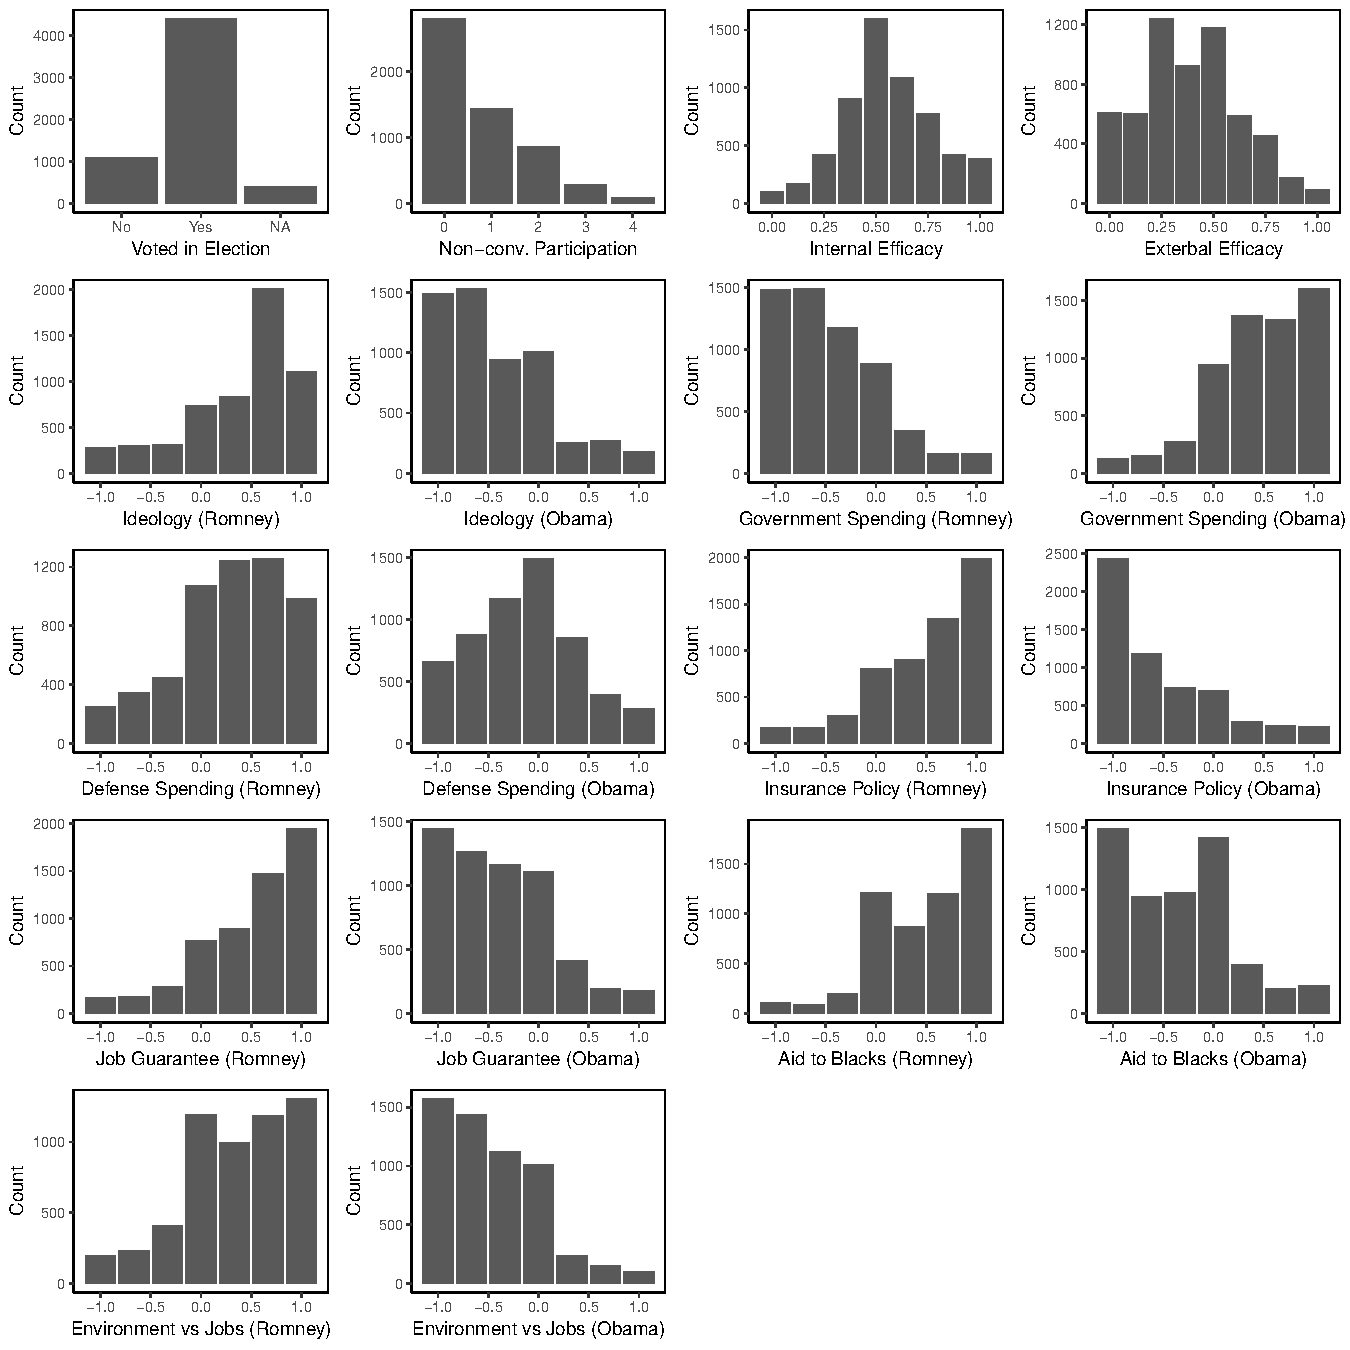
\includegraphics[width=\textwidth]{/data/Dropbox/Uni/Projects/2016/knowledge/fig/descriptives_anes2012dv.pdf}
\caption[Histograms of dependent variables included in 2012 ANES]{Histograms of dependent variables included in 2012 ANES.}\label{fig:descriptives_anes2012dv}
\end{figure}

\begin{figure}[h]\centering
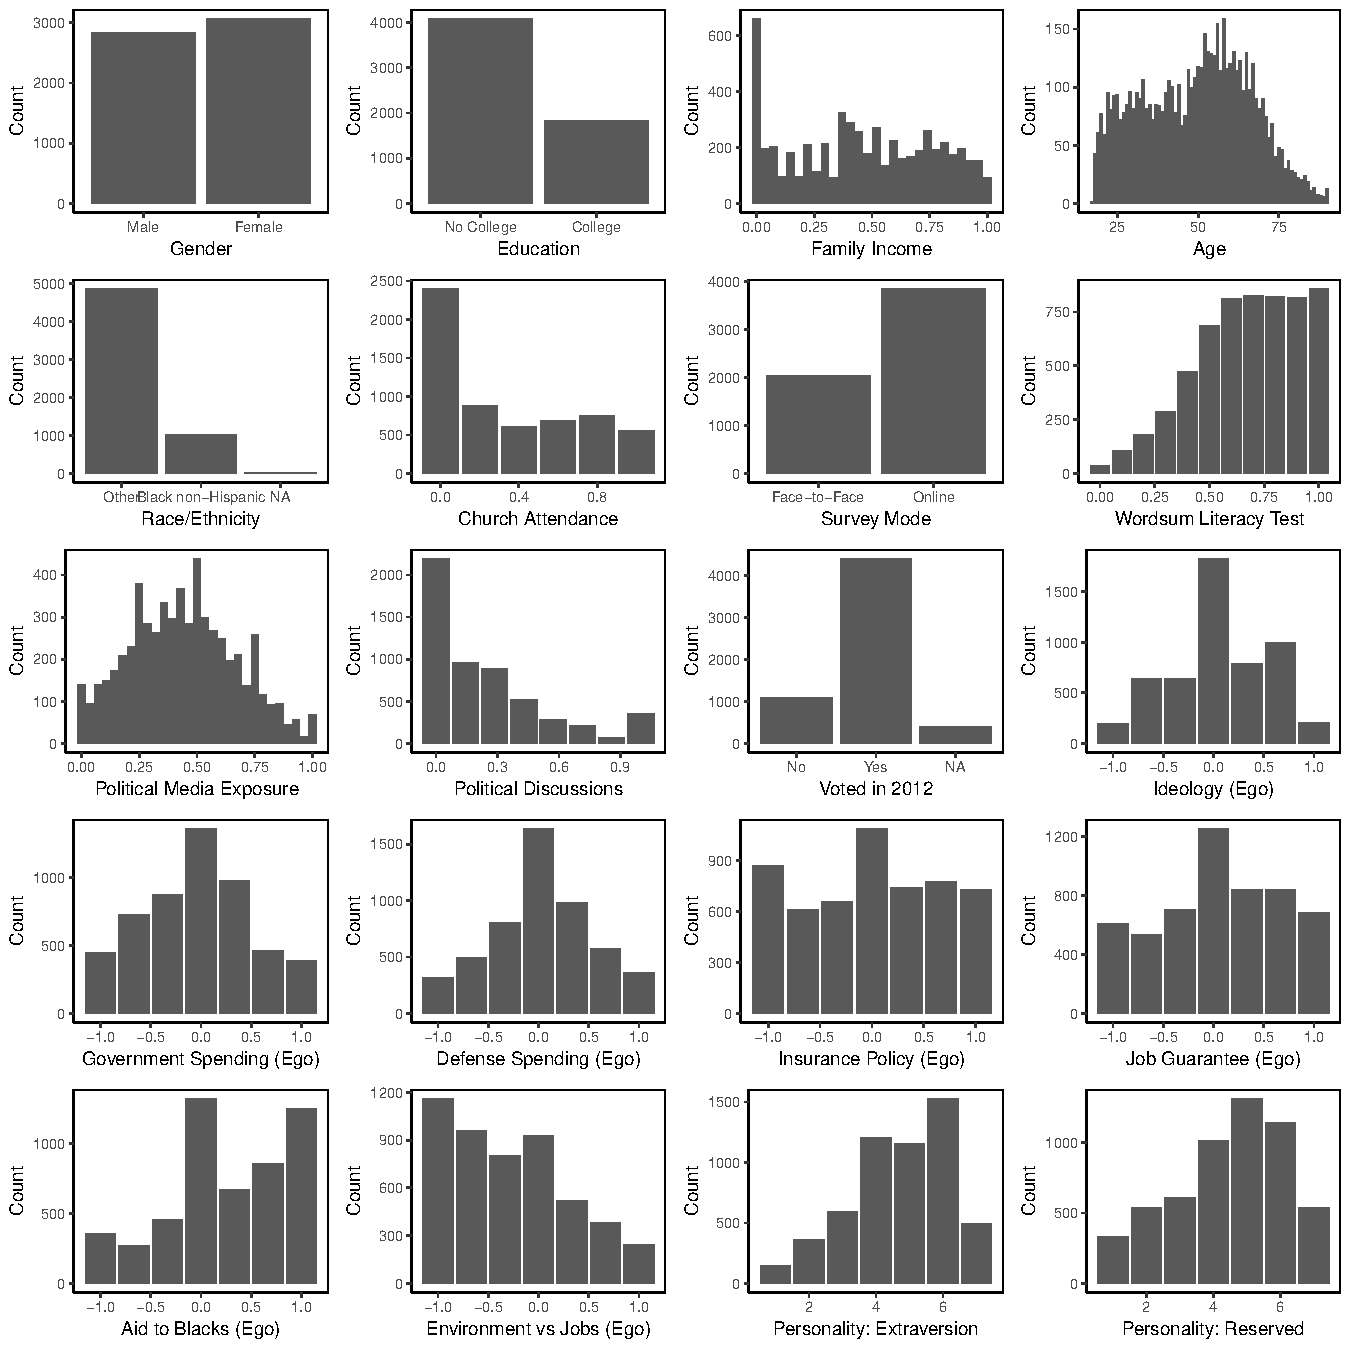
\includegraphics[width=\textwidth]{/data/Dropbox/Uni/Projects/2016/knowledge/fig/descriptives_anes2012iv.pdf}
\caption[Histograms of independent variables included in 2012 ANES]{Histograms of independent variables included in 2012 ANES.}\label{fig:descriptives_anes2012iv}
\end{figure}

\clearpage
\subsection{Variable Distributions -- 2016 ANES}
\begin{figure}[h]\centering
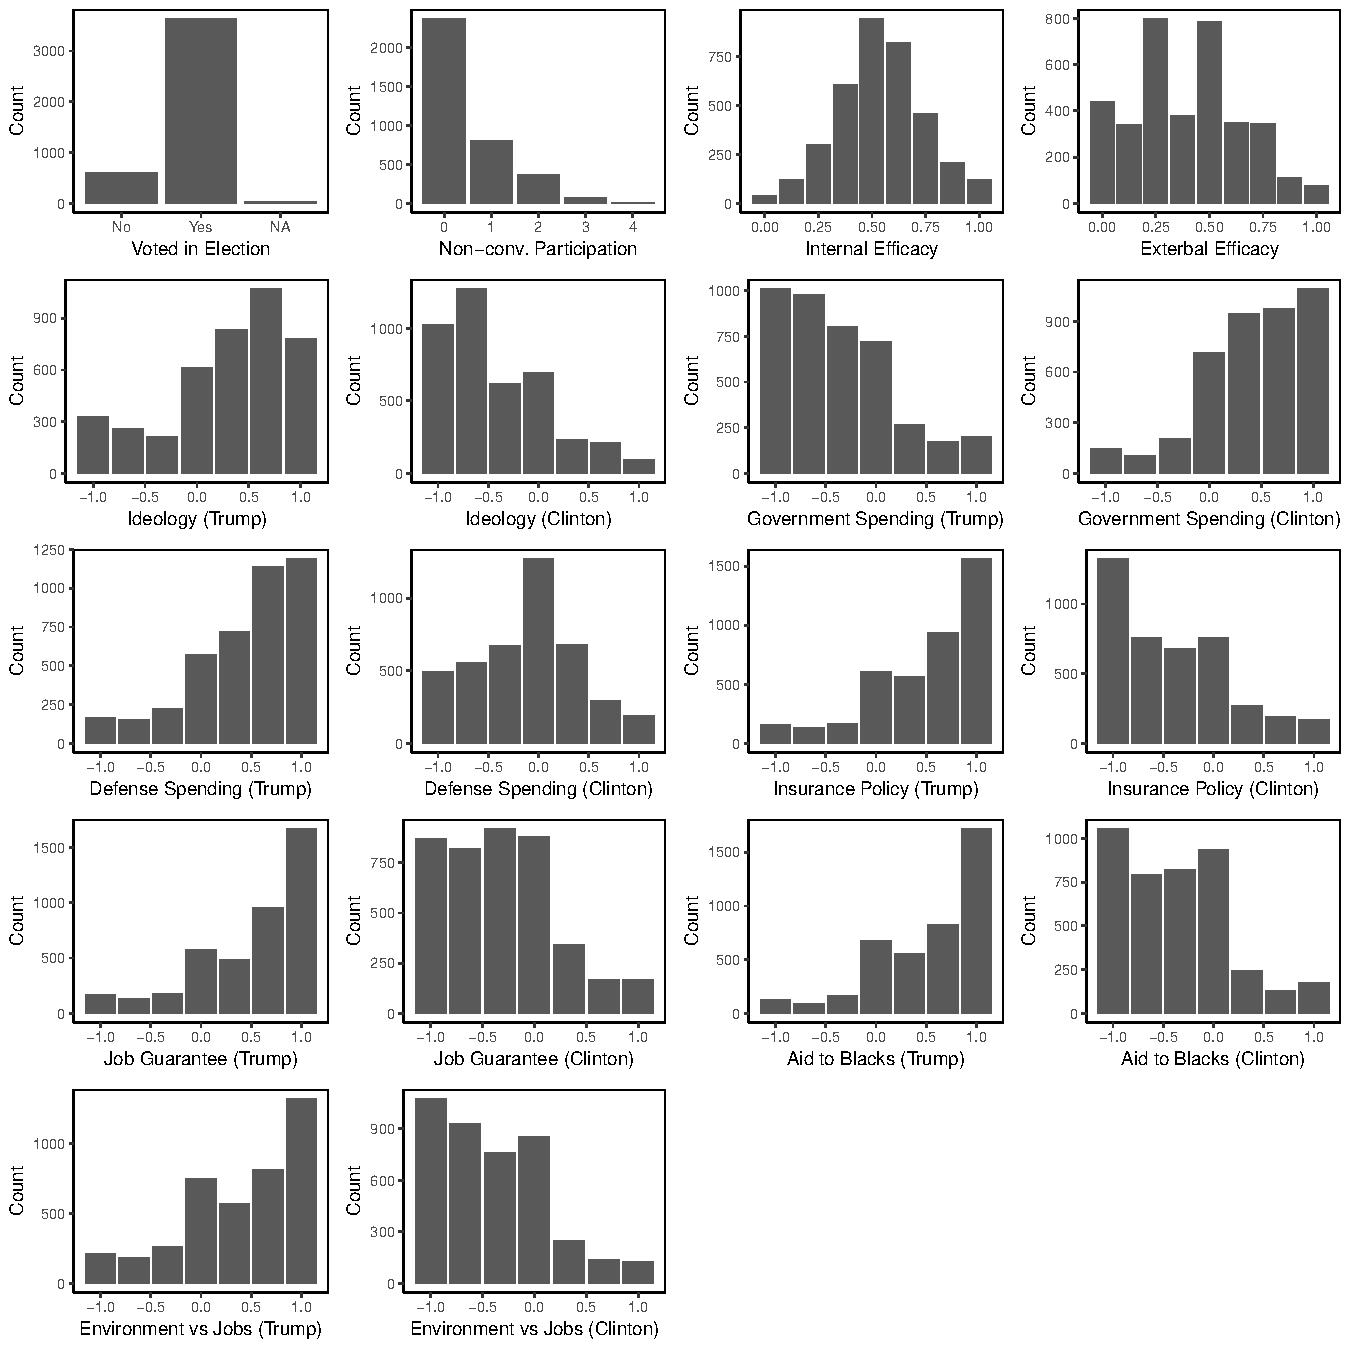
\includegraphics[width=\textwidth]{/data/Dropbox/Uni/Projects/2016/knowledge/fig/descriptives_anes2016dv.pdf}
\caption[Histograms of dependent variables included in 2016 ANES]{Histograms of dependent variables included in 2016 ANES.}\label{fig:descriptives_anes2016dv}
\end{figure}

\begin{figure}[h]\centering
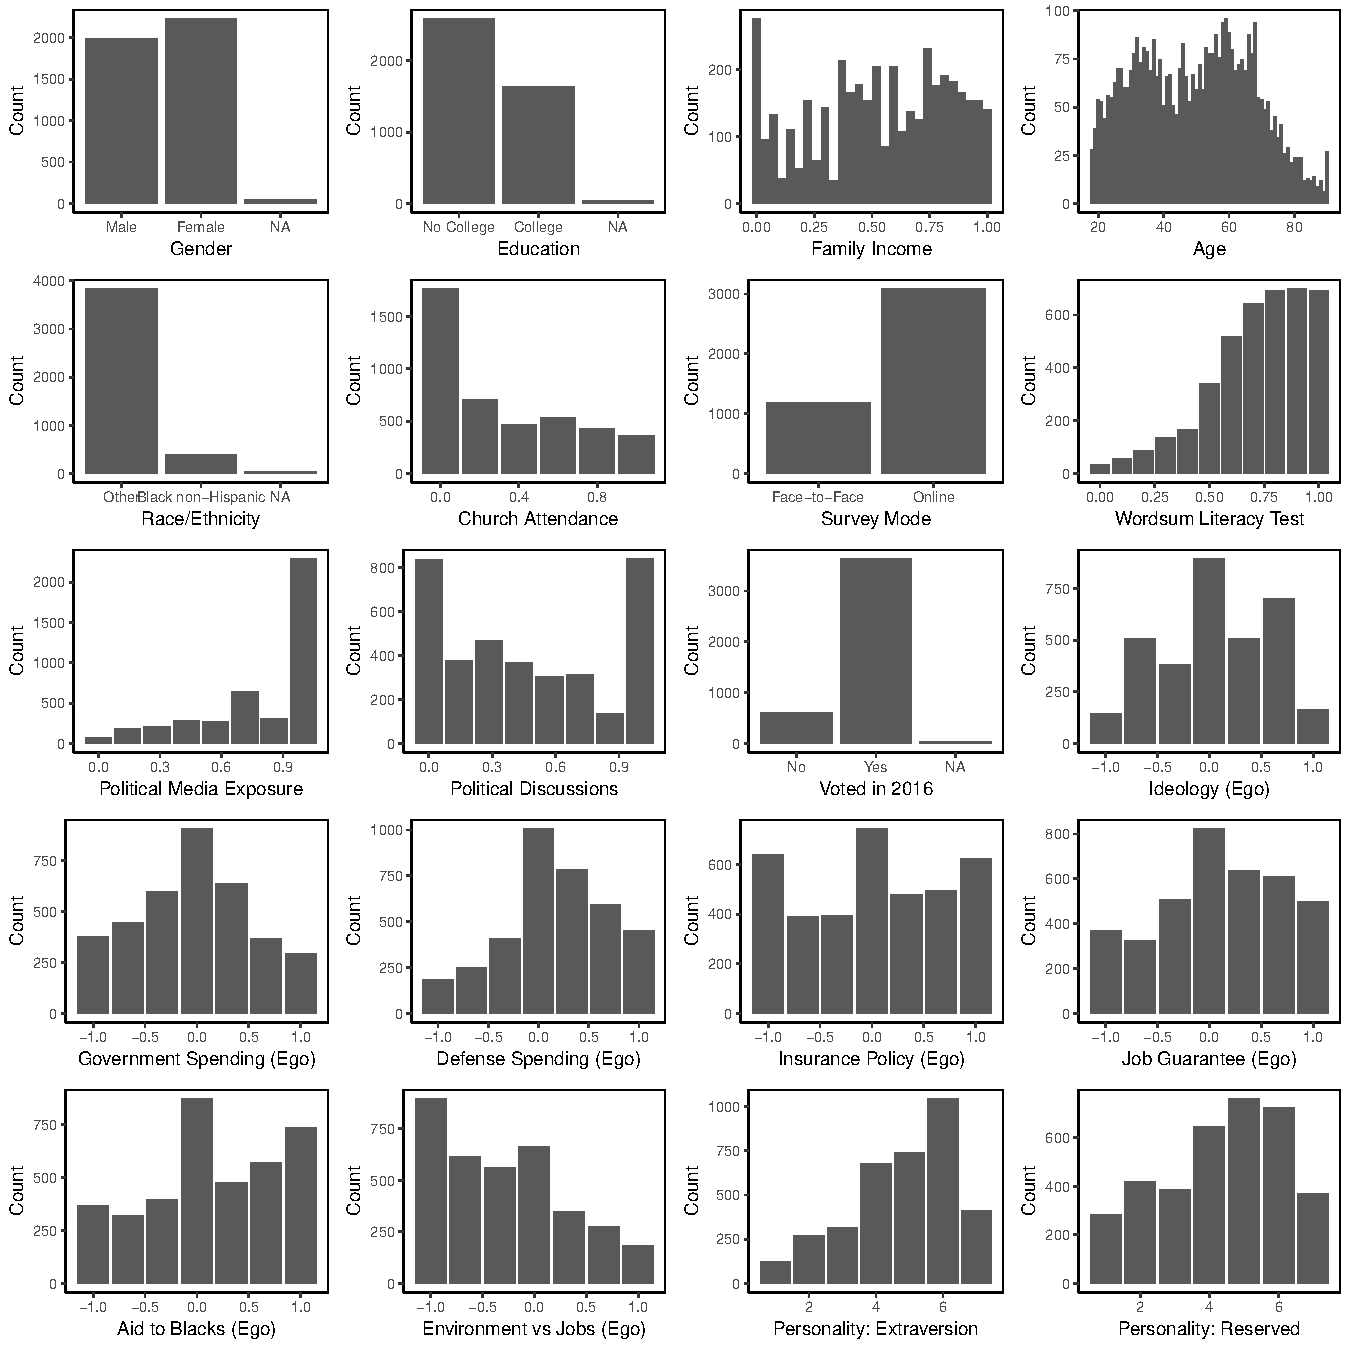
\includegraphics[width=\textwidth]{/data/Dropbox/Uni/Projects/2016/knowledge/fig/descriptives_anes2016iv.pdf}
\caption[Histograms of independent variables included in 2016 ANES]{Histograms of independent variables included in 2016 ANES.}\label{fig:descriptives_anes2016iv}
\end{figure}

\clearpage
\subsection{Variable Distributions -- 2015 YouGov}

\begin{figure}[h]\centering
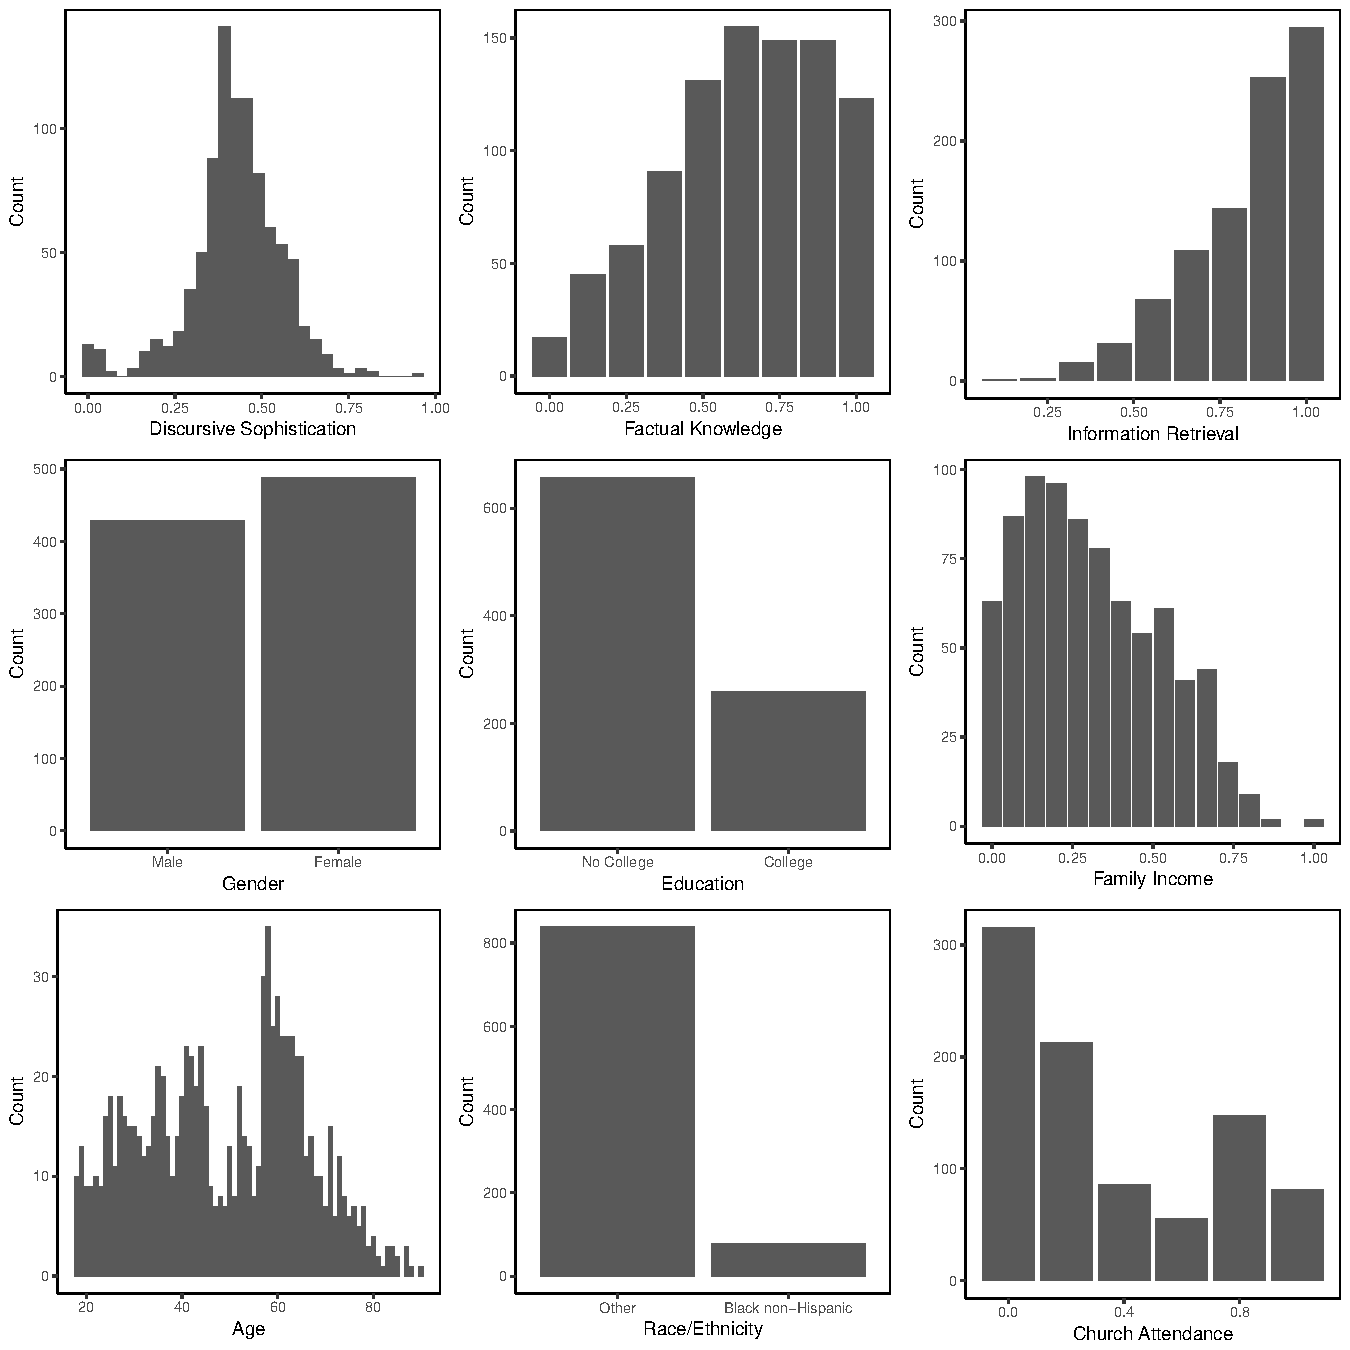
\includegraphics[width=\textwidth]{/data/Dropbox/Uni/Projects/2016/knowledge/fig/descriptives_yg.pdf}
\caption[Histogram of variables included in 2015 YouGov survey]{Histogram of variables included in 2015 YouGov survey.}\label{fig:descriptives_yg}
\end{figure}


\clearpage
\section{Robustness Checks}\label{app:personality}
%\renewcommand\thefigure{D.\arabic{figure}}
%\renewcommand\thetable{D.\arabic{table}}
%\setcounter{figure}{0}
%\setcounter{table}{0}

\subsection{Controlling for Personality Characteristics}
\begin{figure}[h]\centering
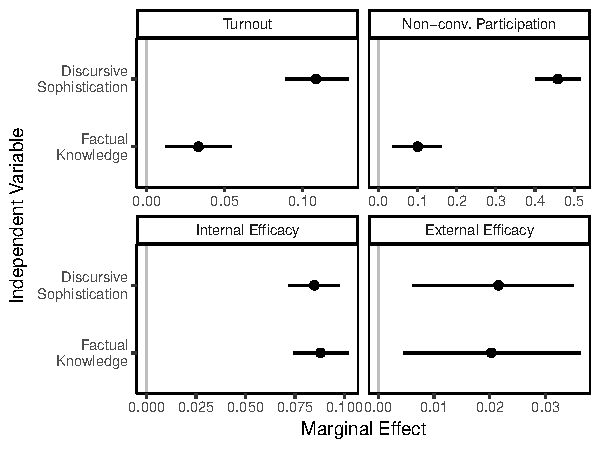
\includegraphics{/data/Dropbox/Uni/Projects/2016/knowledge/fig/knoweff_personality.pdf}
\caption[Effects of sophistication on political engagement controlling for personality characteristics in the 2012 and 2016 ANES]{Effects of sophistication on internal efficacy, external efficacy, non-conventional participation, and turnout in the 2012 and 2016 ANES. For each dependent variable, the figure displays the change in expected values after increasing each sophistication measure from -1 to +1 standard deviation from its mean (including 95\% confidence intervals). Model estimates are based on logistic regression (turnout) or OLS (internal efficacy, external efficacy, non-conventional participation). Both sophistication measure are included simultaneously while controlling for gender, education, income, age, race, church attendance, survey mode, Wordsum vocabulary scores, as well as personality characteristics (extraversion and being reserved). Full model results are presented in the appendix, Tables \ref{tab:knoweff2012_personality} and \ref{tab:knoweff2016_personality}.
}\label{fig:knoweff_personality}
\end{figure}

\clearpage
\subsection{Controlling for Individual Response Length}
\begin{figure}[h]\centering
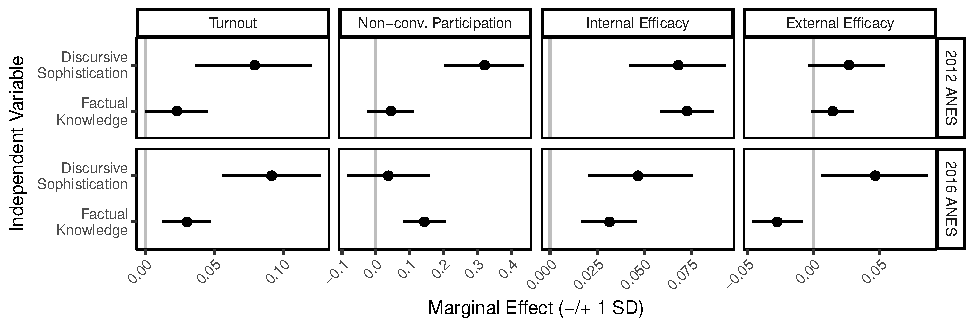
\includegraphics{/data/Dropbox/Uni/Projects/2016/knowledge/fig/knoweff_lwc.pdf}
\caption[Effects of sophistication on political engagement controlling for response length in the 2012 and 2016 ANES]{Effects of sophistication on internal efficacy, external efficacy, non-conventional participation, and turnout in the 2012 and 2016 ANES. For each dependent variable, the figure displays the change in expected values after increasing each sophistication measure from -1 to +1 standard deviation from its mean (including 95\% confidence intervals). Model estimates are based on logistic regression (turnout) or OLS (internal efficacy, external efficacy, non-conventional participation). Both sophistication measure are included simultaneously while controlling for gender, education, income, age, race, church attendance, survey mode, Wordsum vocabulary scores, as well as the logged word count across open-ended responses. Full model results are presented in the appendix, Tables \ref{tab:knoweff2012_lwc} and \ref{tab:knoweff2016_lwc}.
}\label{fig:knoweff_lwc}
\end{figure}


\clearpage
\section{Tables of Model Estimates}
%\renewcommand\thefigure{E.\arabic{figure}}
%\renewcommand\thetable{E.\arabic{table}}
%\setcounter{figure}{0}
%\setcounter{table}{0}

\subsection{Main Analyses}

% Table created by stargazer v.5.2 by Marek Hlavac, Harvard University. E-mail: hlavac at fas.harvard.edu
% Date and time: Thu, Apr 05, 2018 - 12:26:10 AM
% Requires LaTeX packages: dcolumn 
\begin{table}[!htbp] \centering 
  \caption{Effects of sophistication on turnout, non-conventional participation, internal efficacy, 
          and external efficacy in the 2012 ANES. Standard errors in parentheses. Estimates are used for
          Figure 2 in the main text.} 
  \label{tab:knoweff2012} 
\begin{tabular}{@{\extracolsep{0pt}}lD{.}{.}{-3} D{.}{.}{-3} D{.}{.}{-3} D{.}{.}{-3} } 
\\[-1.8ex]\hline 
\hline \\[-1.8ex] 
 & \multicolumn{4}{c}{\textit{Dependent variable:}} \\ 
\cline{2-5} 
 & \multicolumn{1}{c}{Turnout} & \multicolumn{1}{c}{Participation} & \multicolumn{1}{c}{Internal Efficacy} & \multicolumn{1}{c}{External Efficacy} \\ 
\hline \\[-1.8ex] 
 Discursive Soph. & 2.921^{***} & 1.440^{***} & 0.278^{***} & 0.084^{***} \\ 
  & (0.299) & (0.098) & (0.020) & (0.024) \\ 
  Factual Knowledge & 0.432^{*} & 0.099 & 0.158^{***} & 0.032 \\ 
  & (0.218) & (0.075) & (0.016) & (0.018) \\ 
  Female & 0.086 & -0.067^{*} & -0.053^{***} & 0.016^{*} \\ 
  & (0.085) & (0.028) & (0.006) & (0.007) \\ 
  College Degree & 0.350^{**} & 0.159^{***} & 0.022^{**} & 0.035^{***} \\ 
  & (0.112) & (0.034) & (0.007) & (0.008) \\ 
  Family Income & 0.947^{***} & 0.022 & 0.010 & 0.016 \\ 
  & (0.156) & (0.052) & (0.011) & (0.013) \\ 
  Age (log) & 0.988^{***} & 0.102^{**} & -0.006 & -0.014 \\ 
  & (0.105) & (0.038) & (0.008) & (0.009) \\ 
  African American & 0.910^{***} & 0.096^{*} & 0.066^{***} & 0.082^{***} \\ 
  & (0.123) & (0.038) & (0.008) & (0.009) \\ 
  Church Attendance & 0.752^{***} & 0.112^{**} & 0.010 & 0.048^{***} \\ 
  & (0.129) & (0.040) & (0.008) & (0.010) \\ 
  Mode: Online & 0.530^{***} & 0.227^{***} & 0.017^{*} & -0.039^{***} \\ 
  & (0.094) & (0.033) & (0.007) & (0.008) \\ 
  Wordsum Score & 0.638^{**} & 0.403^{***} & 0.092^{***} & 0.013 \\ 
  & (0.219) & (0.076) & (0.016) & (0.019) \\ 
  Constant & -5.019^{***} & -0.598^{***} & 0.326^{***} & 0.352^{***} \\ 
  & (0.401) & (0.145) & (0.030) & (0.035) \\ 
 \hline \\[-1.8ex] 
Observations & \multicolumn{1}{c}{4,716} & \multicolumn{1}{c}{4,692} & \multicolumn{1}{c}{4,996} & \multicolumn{1}{c}{4,985} \\ 
R$^{2}$ &  & \multicolumn{1}{c}{0.124} & \multicolumn{1}{c}{0.161} & \multicolumn{1}{c}{0.043} \\ 
Log Likelihood & \multicolumn{1}{c}{-1,868.199} &  &  &  \\ 
\hline 
\hline \\[-1.8ex] 
\textit{Note:}  & \multicolumn{4}{r}{$^{*}$p$<$0.05; $^{**}$p$<$0.01; $^{***}$p$<$0.001} \\ 
\end{tabular} 
\end{table} 


% Table created by stargazer v.5.2 by Marek Hlavac, Harvard University. E-mail: hlavac at fas.harvard.edu
% Date and time: Tue, Apr 03, 2018 - 12:07:45 AM
% Requires LaTeX packages: dcolumn 
\begin{table}[!htbp] \centering 
  \caption{Effects of sophistication on turnout, non-conventional participation, internal efficacy, 
          and external efficacy in the 2016 ANES. Standard errors in parentheses. Estimates are used for
          Figure 2 in the main text.} 
  \label{tab:knoweff2016} 
\begin{tabular}{@{\extracolsep{0pt}}lD{.}{.}{-3} D{.}{.}{-3} D{.}{.}{-3} D{.}{.}{-3} } 
\\[-1.8ex]\hline 
\hline \\[-1.8ex] 
 & \multicolumn{4}{c}{\textit{Dependent variable:}} \\ 
\cline{2-5} 
 & \multicolumn{1}{c}{Turnout} & \multicolumn{1}{c}{Participation} & \multicolumn{1}{c}{Internal Efficacy} & \multicolumn{1}{c}{External Efficacy} \\ 
\hline \\[-1.8ex] 
 Discursive Soph. & 3.748^{***} & 0.790^{***} & 0.220^{***} & 0.087^{*} \\ 
  & (0.485) & (0.131) & (0.031) & (0.041) \\ 
  Factual Knowledge & 0.733^{***} & 0.271^{***} & 0.059^{***} & -0.052^{**} \\ 
  & (0.219) & (0.058) & (0.014) & (0.018) \\ 
  Female & 0.177 & 0.061^{*} & -0.060^{***} & -0.003 \\ 
  & (0.114) & (0.029) & (0.007) & (0.009) \\ 
  College Degree & 0.556^{***} & 0.091^{**} & 0.058^{***} & 0.056^{***} \\ 
  & (0.141) & (0.033) & (0.008) & (0.010) \\ 
  Family Income & 0.497^{*} & -0.075 & 0.021 & 0.062^{***} \\ 
  & (0.207) & (0.055) & (0.013) & (0.017) \\ 
  Age (log) & 0.837^{***} & -0.111^{**} & 0.020^{*} & -0.005 \\ 
  & (0.139) & (0.038) & (0.009) & (0.012) \\ 
  African American & 1.124^{***} & 0.097 & 0.057^{***} & -0.020 \\ 
  & (0.237) & (0.051) & (0.012) & (0.016) \\ 
  Church Attendance & 1.069^{***} & -0.175^{***} & -0.006 & 0.080^{***} \\ 
  & (0.191) & (0.043) & (0.010) & (0.014) \\ 
  Mode: Online & 0.183 & 0.113^{**} & 0.068^{***} & -0.015 \\ 
  & (0.136) & (0.036) & (0.009) & (0.011) \\ 
  Wordsum Score & 0.934^{***} & 0.399^{***} & 0.103^{***} & 0.015 \\ 
  & (0.275) & (0.079) & (0.019) & (0.025) \\ 
  Constant & -4.235^{***} & 0.213 & 0.233^{***} & 0.336^{***} \\ 
  & (0.534) & (0.151) & (0.036) & (0.048) \\ 
 \hline \\[-1.8ex] 
Observations & \multicolumn{1}{c}{3,487} & \multicolumn{1}{c}{3,040} & \multicolumn{1}{c}{3,038} & \multicolumn{1}{c}{3,039} \\ 
R$^{2}$ &  & \multicolumn{1}{c}{0.062} & \multicolumn{1}{c}{0.147} & \multicolumn{1}{c}{0.043} \\ 
Log Likelihood & \multicolumn{1}{c}{-1,087.769} &  &  &  \\ 
\hline 
\hline \\[-1.8ex] 
\textit{Note:}  & \multicolumn{4}{r}{$^{*}$p$<$0.05; $^{**}$p$<$0.01; $^{***}$p$<$0.001} \\ 
\end{tabular} 
\end{table} 


% Table created by stargazer v.5.2.3 by Marek Hlavac, Social Policy Institute. E-mail: marek.hlavac at gmail.com
% Date and time: Mon, Aug 15, 2022 - 10:21:41 PM
% Requires LaTeX packages: dcolumn 
\begin{table}[!htbp] \centering 
  \caption{Linear regressions predicting information retrieval in the 2015 YouGov study.
          Standard errors in parentheses. Estimates are used for Figure \ref{fig:yg_disease}
          in the main text.} 
  \label{tab:yg_disease} 
\footnotesize 
\begin{tabular}{@{\extracolsep{-25pt}}lD{.}{.}{-3} D{.}{.}{-3} D{.}{.}{-3} } 
\\[-1.8ex]\hline 
\hline \\[-1.8ex] 
 & \multicolumn{3}{c}{\textit{Dependent variable:}} \\ 
\cline{2-4} 
 & \multicolumn{3}{c}{Information Retrieval} \\ 
\\[-1.8ex] & \multicolumn{1}{c}{(1)} & \multicolumn{1}{c}{(2)} & \multicolumn{1}{c}{(3)}\\ 
\hline \\[-1.8ex] 
 Discursive Soph. & 0.039^{***} & 0.033^{***} & 0.032^{***} \\ 
  & (0.006) & (0.006) & (0.006) \\ 
  Factual Knowledge & 0.030^{***} & 0.035^{***} & 0.034^{***} \\ 
  & (0.006) & (0.007) & (0.007) \\ 
  Disc. X Factual &  &  & -0.008 \\ 
  &  &  & (0.006) \\ 
  Female &  & 0.043^{***} & 0.043^{***} \\ 
  &  & (0.012) & (0.012) \\ 
  Age &  & 0.001^{*} & 0.001^{*} \\ 
  &  & (0.0004) & (0.0004) \\ 
  Black &  & -0.027 & -0.026 \\ 
  &  & (0.021) & (0.021) \\ 
  College Degree &  & 0.017 & 0.017 \\ 
  &  & (0.014) & (0.014) \\ 
  Household Income &  & -0.061^{*} & -0.060^{*} \\ 
  &  & (0.030) & (0.030) \\ 
  Church Attendance &  & -0.059^{***} & -0.059^{***} \\ 
  &  & (0.017) & (0.017) \\ 
  Constant & 0.828^{***} & 0.807^{***} & 0.811^{***} \\ 
  & (0.005) & (0.021) & (0.021) \\ 
 \hline \\[-1.8ex] 
Observations & \multicolumn{1}{c}{918} & \multicolumn{1}{c}{792} & \multicolumn{1}{c}{792} \\ 
R$^{2}$ & \multicolumn{1}{c}{0.100} & \multicolumn{1}{c}{0.137} & \multicolumn{1}{c}{0.139} \\ 
\hline 
\hline \\[-1.8ex] 
\textit{Note:}  & \multicolumn{3}{r}{$^{*}$p$<$0.05; $^{**}$p$<$0.01; $^{***}$p$<$0.001} \\ 
\end{tabular} 
\end{table} 


% Table created by stargazer v.5.2 by Marek Hlavac, Harvard University. E-mail: hlavac at fas.harvard.edu
% Date and time: Mon, Apr 02, 2018 - 03:43:21 PM
% Requires LaTeX packages: dcolumn 
\begin{table}[!htbp] \centering 
  \caption{Effects of gender on discursive sophistication and factual knowledge in the 
          2012 ANES and 2016 ANES. Standard errors in parentheses. Estimates are used for 
          Figure 8 in the main text.} 
  \label{tab:determinants_anes} 
\begin{tabular}{@{\extracolsep{0pt}}lD{.}{.}{-3} D{.}{.}{-3} D{.}{.}{-3} D{.}{.}{-3} } 
\\[-1.8ex]\hline 
\hline \\[-1.8ex] 
 & \multicolumn{4}{c}{\textit{Dependent variable:}} \\ 
\cline{2-5} 
\\[-1.8ex] & \multicolumn{2}{c}{Discursive Sophistication} & \multicolumn{2}{c}{Factual Knowledge} \\ 
 & \multicolumn{1}{c}{2012 ANES} & \multicolumn{1}{c}{2016 ANES} & \multicolumn{1}{c}{2012 ANES} & \multicolumn{1}{c}{2016 ANES} \\ 
\hline \\[-1.8ex] 
 Female & 0.003 & -0.003 & -0.050^{***} & -0.031^{**} \\ 
  & (0.004) & (0.004) & (0.006) & (0.010) \\ 
  Media Exposure & 0.042^{***} & 0.046^{***} & 0.067^{***} & 0.075^{***} \\ 
  & (0.010) & (0.009) & (0.014) & (0.021) \\ 
  Discussion Freqency & 0.119^{***} & 0.040^{***} & 0.062^{***} & 0.061^{***} \\ 
  & (0.007) & (0.007) & (0.010) & (0.015) \\ 
  College Degree & 0.070^{***} & 0.046^{***} & 0.091^{***} & 0.047^{***} \\ 
  & (0.005) & (0.005) & (0.007) & (0.010) \\ 
  Family Income & 0.052^{***} & 0.033^{***} & 0.116^{***} & 0.088^{***} \\ 
  & (0.008) & (0.008) & (0.010) & (0.018) \\ 
  Age (log) & 0.017^{**} & -0.002 & 0.081^{***} & 0.091^{***} \\ 
  & (0.006) & (0.006) & (0.008) & (0.014) \\ 
  African American & -0.005 & -0.034^{***} & -0.085^{***} & -0.004 \\ 
  & (0.005) & (0.008) & (0.008) & (0.017) \\ 
  Church Attendance & 0.004 & 0.004 & -0.003 & -0.017 \\ 
  & (0.006) & (0.006) & (0.008) & (0.014) \\ 
  Mode: Online & -0.045^{***} & -0.122^{***} & 0.092^{***} & 0.086^{***} \\ 
  & (0.005) & (0.005) & (0.006) & (0.011) \\ 
  Constant & 0.192^{***} & 0.323^{***} & 0.195^{***} & 0.016 \\ 
  & (0.021) & (0.022) & (0.030) & (0.051) \\ 
 \hline \\[-1.8ex] 
Observations & \multicolumn{1}{c}{4,690} & \multicolumn{1}{c}{2,611} & \multicolumn{1}{c}{4,690} & \multicolumn{1}{c}{2,602} \\ 
R$^{2}$ & \multicolumn{1}{c}{0.178} & \multicolumn{1}{c}{0.270} & \multicolumn{1}{c}{0.282} & \multicolumn{1}{c}{0.106} \\ 
\hline 
\hline \\[-1.8ex] 
\textit{Note:}  & \multicolumn{4}{r}{$^{*}$p$<$0.05; $^{**}$p$<$0.01; $^{***}$p$<$0.001} \\ 
\end{tabular} 
\end{table} 


% Table created by stargazer v.5.2 by Marek Hlavac, Harvard University. E-mail: hlavac at fas.harvard.edu
% Date and time: Mon, Apr 02, 2018 - 07:34:30 PM
% Requires LaTeX packages: dcolumn 
\begin{table}[!htbp] \centering 
  \caption{Effects of gender on discursive sophistication and factual knowledge in the 
          2015 YouGov Study. Standard errors in parentheses. Estimates are used for 
          Figure 8 in the main text.} 
  \label{tab:determinants_yg} 
\begin{tabular}{@{\extracolsep{0pt}}lD{.}{.}{-3} D{.}{.}{-3} } 
\\[-1.8ex]\hline 
\hline \\[-1.8ex] 
 & \multicolumn{2}{c}{\textit{Dependent variable:}} \\ 
\cline{2-3} 
 & \multicolumn{1}{c}{Discursive Sophistication} & \multicolumn{1}{c}{Factual Knowledge} \\ 
\hline \\[-1.8ex] 
 Female & 0.011 & -0.157^{***} \\ 
  & (0.009) & (0.016) \\ 
  College Degree & 0.030^{**} & 0.108^{***} \\ 
  & (0.011) & (0.019) \\ 
  Family Income & -0.017 & 0.233^{***} \\ 
  & (0.023) & (0.041) \\ 
  Age (log) & 0.044^{***} & 0.135^{***} \\ 
  & (0.012) & (0.021) \\ 
  African American & -0.063^{***} & -0.086^{**} \\ 
  & (0.017) & (0.029) \\ 
  Church Attendance & -0.006 & -0.051^{*} \\ 
  & (0.013) & (0.023) \\ 
  Constant & 0.258^{***} & 0.125 \\ 
  & (0.047) & (0.083) \\ 
 \hline \\[-1.8ex] 
Observations & \multicolumn{1}{c}{792} & \multicolumn{1}{c}{792} \\ 
R$^{2}$ & \multicolumn{1}{c}{0.048} & \multicolumn{1}{c}{0.272} \\ 
\hline 
\hline \\[-1.8ex] 
\textit{Note:}  & \multicolumn{2}{r}{$^{*}$p$<$0.05; $^{**}$p$<$0.01; $^{***}$p$<$0.001} \\ 
\end{tabular} 
\end{table} 


\clearpage
\subsection{Robustness Checks}

% Table created by stargazer v.5.2 by Marek Hlavac, Harvard University. E-mail: hlavac at fas.harvard.edu
% Date and time: Mon, Apr 02, 2018 - 03:53:40 PM
% Requires LaTeX packages: dcolumn 
\begin{table}[!htbp] \centering 
  \caption{Effects of sophistication on turnout, non-conventional participation, internal efficacy, 
          and external efficacy controlling for personality characteristics in the 2012 ANES. 
          Standard errors in parentheses. Estimates are used for Figure \ref{fig:knoweff_personality} 
          in the appendix.} 
  \label{tab:knoweff2012_personality} 
\begin{tabular}{@{\extracolsep{0pt}}lD{.}{.}{-3} D{.}{.}{-3} D{.}{.}{-3} D{.}{.}{-3} } 
\\[-1.8ex]\hline 
\hline \\[-1.8ex] 
 & \multicolumn{4}{c}{\textit{Dependent variable:}} \\ 
\cline{2-5} 
 & \multicolumn{1}{c}{Turnout} & \multicolumn{1}{c}{Participation} & \multicolumn{1}{c}{Internal Efficacy} & \multicolumn{1}{c}{External Efficacy} \\ 
\hline \\[-1.8ex] 
 Discursive Soph. & 2.967^{***} & 1.432^{***} & 0.275^{***} & 0.095^{***} \\ 
  & (0.305) & (0.100) & (0.021) & (0.025) \\ 
  Factual Knowledge & 0.441^{*} & 0.105 & 0.165^{***} & 0.035 \\ 
  & (0.218) & (0.075) & (0.016) & (0.019) \\ 
  Female & 0.085 & -0.080^{**} & -0.060^{***} & 0.009 \\ 
  & (0.085) & (0.028) & (0.006) & (0.007) \\ 
  College Degree & 0.350^{**} & 0.160^{***} & 0.020^{**} & 0.032^{***} \\ 
  & (0.112) & (0.034) & (0.007) & (0.008) \\ 
  Family Income & 0.946^{***} & -0.0001 & 0.006 & 0.010 \\ 
  & (0.157) & (0.052) & (0.011) & (0.013) \\ 
  Age (log) & 0.981^{***} & 0.102^{**} & -0.003 & -0.017 \\ 
  & (0.106) & (0.039) & (0.008) & (0.010) \\ 
  African American & 0.893^{***} & 0.093^{*} & 0.066^{***} & 0.077^{***} \\ 
  & (0.124) & (0.038) & (0.008) & (0.010) \\ 
  Church Attendance & 0.728^{***} & 0.103^{**} & 0.006 & 0.044^{***} \\ 
  & (0.130) & (0.040) & (0.008) & (0.010) \\ 
  Mode: Online & 0.544^{***} & 0.251^{***} & 0.022^{**} & -0.032^{***} \\ 
  & (0.096) & (0.033) & (0.007) & (0.008) \\ 
  Wordsum Score & 0.643^{**} & 0.409^{***} & 0.092^{***} & 0.020 \\ 
  & (0.220) & (0.076) & (0.016) & (0.019) \\ 
  Extraversion & 0.031 & 0.033^{***} & 0.009^{***} & 0.020^{***} \\ 
  & (0.030) & (0.010) & (0.002) & (0.002) \\ 
  Reserved & 0.009 & -0.023^{**} & -0.005^{**} & 0.002 \\ 
  & (0.026) & (0.009) & (0.002) & (0.002) \\ 
  Constant & -5.185^{***} & -0.638^{***} & 0.297^{***} & 0.254^{***} \\ 
  & (0.450) & (0.158) & (0.034) & (0.039) \\ 
 \hline \\[-1.8ex] 
Observations & \multicolumn{1}{c}{4,691} & \multicolumn{1}{c}{4,685} & \multicolumn{1}{c}{4,691} & \multicolumn{1}{c}{4,679} \\ 
R$^{2}$ &  & \multicolumn{1}{c}{0.128} & \multicolumn{1}{c}{0.171} & \multicolumn{1}{c}{0.059} \\ 
Log Likelihood & \multicolumn{1}{c}{-1,861.487} &  &  &  \\ 
\hline 
\hline \\[-1.8ex] 
\textit{Note:}  & \multicolumn{4}{r}{$^{*}$p$<$0.05; $^{**}$p$<$0.01; $^{***}$p$<$0.001} \\ 
\end{tabular} 
\end{table} 


% Table created by stargazer v.5.2 by Marek Hlavac, Harvard University. E-mail: hlavac at fas.harvard.edu
% Date and time: Thu, Apr 05, 2018 - 07:38:52 AM
% Requires LaTeX packages: dcolumn 
\begin{table}[!htbp] \centering 
  \caption{Effects of sophistication on turnout, non-conventional participation, internal efficacy, 
          and external efficacy controlling for personality characteristics in the 2016 ANES. 
          Standard errors in parentheses. Estimates are used for Figure \ref{fig:knoweff_personality} 
          in the appendix.} 
  \label{tab:knoweff2016_personality} 
\begin{tabular}{@{\extracolsep{0pt}}lD{.}{.}{-3} D{.}{.}{-3} D{.}{.}{-3} D{.}{.}{-3} } 
\\[-1.8ex]\hline 
\hline \\[-1.8ex] 
 & \multicolumn{4}{c}{\textit{Dependent variable:}} \\ 
\cline{2-5} 
 & \multicolumn{1}{c}{Turnout} & \multicolumn{1}{c}{Participation} & \multicolumn{1}{c}{Internal Efficacy} & \multicolumn{1}{c}{External Efficacy} \\ 
\hline \\[-1.8ex] 
 Discursive Soph. & 3.936^{***} & 0.760^{***} & 0.213^{***} & 0.070 \\ 
  & (0.543) & (0.132) & (0.031) & (0.042) \\ 
  Factual Knowledge & 0.717^{**} & 0.260^{***} & 0.056^{***} & -0.052^{**} \\ 
  & (0.241) & (0.059) & (0.014) & (0.019) \\ 
  Female & 0.172 & 0.046 & -0.064^{***} & -0.004 \\ 
  & (0.125) & (0.029) & (0.007) & (0.009) \\ 
  College Degree & 0.616^{***} & 0.085^{**} & 0.056^{***} & 0.055^{***} \\ 
  & (0.155) & (0.033) & (0.008) & (0.010) \\ 
  Family Income & 0.471^{*} & -0.085 & 0.017 & 0.060^{***} \\ 
  & (0.230) & (0.055) & (0.013) & (0.017) \\ 
  Age (log) & 0.894^{***} & -0.119^{**} & 0.018^{*} & -0.010 \\ 
  & (0.153) & (0.039) & (0.009) & (0.012) \\ 
  African American & 1.228^{***} & 0.102^{*} & 0.057^{***} & -0.026 \\ 
  & (0.267) & (0.052) & (0.012) & (0.016) \\ 
  Church Attendance & 0.930^{***} & -0.172^{***} & -0.007 & 0.078^{***} \\ 
  & (0.205) & (0.043) & (0.010) & (0.014) \\ 
  Mode: Online & 0.199 & 0.111^{**} & 0.069^{***} & -0.015 \\ 
  & (0.148) & (0.036) & (0.009) & (0.011) \\ 
  Wordsum Score & 0.999^{**} & 0.436^{***} & 0.114^{***} & 0.022 \\ 
  & (0.311) & (0.080) & (0.019) & (0.025) \\ 
  Extraversion & 0.090^{*} & 0.023^{*} & 0.011^{***} & 0.012^{***} \\ 
  & (0.041) & (0.010) & (0.002) & (0.003) \\ 
  Reserved & 0.005 & -0.013 & -0.002 & 0.005 \\ 
  & (0.037) & (0.009) & (0.002) & (0.003) \\ 
  Constant & -4.948^{***} & 0.196 & 0.199^{***} & 0.277^{***} \\ 
  & (0.646) & (0.163) & (0.039) & (0.051) \\ 
 \hline \\[-1.8ex] 
Observations & \multicolumn{1}{c}{2,999} & \multicolumn{1}{c}{3,011} & \multicolumn{1}{c}{3,012} & \multicolumn{1}{c}{3,012} \\ 
R$^{2}$ &  & \multicolumn{1}{c}{0.065} & \multicolumn{1}{c}{0.155} & \multicolumn{1}{c}{0.047} \\ 
Log Likelihood & \multicolumn{1}{c}{-907.430} &  &  &  \\ 
\hline 
\hline \\[-1.8ex] 
\textit{Note:}  & \multicolumn{4}{r}{$^{*}$p$<$0.05; $^{**}$p$<$0.01; $^{***}$p$<$0.001} \\ 
\end{tabular} 
\end{table} 


% Table created by stargazer v.5.2 by Marek Hlavac, Harvard University. E-mail: hlavac at fas.harvard.edu
% Date and time: Thu, Apr 19, 2018 - 11:39:47 PM
% Requires LaTeX packages: dcolumn 
\begin{table}[!htbp] \centering 
  \caption{Effects of sophistication on turnout, non-conventional participation, internal efficacy, 
          and external efficacy controlling for individual response length in the 2012 ANES. 
          Standard errors in parentheses. Estimates are used for Figure \ref{fig:knoweff_lwc} 
          in the appendix.} 
  \label{tab:knoweff2012_lwc} 
\begin{tabular}{@{\extracolsep{0pt}}lD{.}{.}{-3} D{.}{.}{-3} D{.}{.}{-3} D{.}{.}{-3} } 
\\[-1.8ex]\hline 
\hline \\[-1.8ex] 
 & \multicolumn{4}{c}{\textit{Dependent variable:}} \\ 
\cline{2-5} 
 & \multicolumn{1}{c}{Turnout} & \multicolumn{1}{c}{Participation} & \multicolumn{1}{c}{Internal Efficacy} & \multicolumn{1}{c}{External Efficacy} \\ 
\hline \\[-1.8ex] 
 Discursive Soph. & 2.053 & 0.967 & 0.215 & 0.082 \\ 
  & (0.543) & (0.186) & (0.039) & (0.045) \\ 
  Factual Knowledge & 0.426 & 0.096 & 0.158 & 0.032 \\ 
  & (0.218) & (0.075) & (0.016) & (0.018) \\ 
  Female & 0.067 & -0.076 & -0.054 & 0.016 \\ 
  & (0.085) & (0.028) & (0.006) & (0.007) \\ 
  College Degree & 0.370 & 0.167 & 0.023 & 0.035 \\ 
  & (0.113) & (0.034) & (0.007) & (0.008) \\ 
  Family Income & 0.948 & 0.026 & 0.011 & 0.016 \\ 
  & (0.156) & (0.052) & (0.011) & (0.013) \\ 
  Age (log) & 0.976 & 0.094 & -0.007 & -0.014 \\ 
  & (0.106) & (0.039) & (0.008) & (0.009) \\ 
  African American & 0.896 & 0.088 & 0.064 & 0.082 \\ 
  & (0.123) & (0.038) & (0.008) & (0.009) \\ 
  Church Attendance & 0.758 & 0.113 & 0.010 & 0.048 \\ 
  & (0.129) & (0.040) & (0.008) & (0.010) \\ 
  Mode: Online & 0.574 & 0.246 & 0.020 & -0.039 \\ 
  & (0.097) & (0.034) & (0.007) & (0.008) \\ 
  Wordsum Score & 0.626 & 0.396 & 0.091 & 0.013 \\ 
  & (0.219) & (0.076) & (0.016) & (0.019) \\ 
  Word Count (log) & 0.970 & 0.539 & 0.071 & 0.003 \\ 
  & (0.507) & (0.180) & (0.037) & (0.044) \\ 
  Constant & -5.237 & -0.710 & 0.311 & 0.352 \\ 
  & (0.418) & (0.150) & (0.031) & (0.036) \\ 
 \hline \\[-1.8ex] 
Observations & \multicolumn{1}{c}{4,716} & \multicolumn{1}{c}{4,692} & \multicolumn{1}{c}{4,996} & \multicolumn{1}{c}{4,985} \\ 
R$^{2}$ &  & \multicolumn{1}{c}{0.126} & \multicolumn{1}{c}{0.162} & \multicolumn{1}{c}{0.043} \\ 
Log Likelihood & \multicolumn{1}{c}{-1,866.366} &  &  &  \\ 
\hline 
\hline \\[-1.8ex] 
\end{tabular} 
\end{table} 


% Table created by stargazer v.5.2 by Marek Hlavac, Harvard University. E-mail: hlavac at fas.harvard.edu
% Date and time: Mon, Apr 02, 2018 - 12:18:45 PM
% Requires LaTeX packages: dcolumn 
\begin{table}[!htbp] \centering 
  \caption{Effects of sophistication on turnout, non-conventional participation, internal efficacy, 
          and external efficacy controlling for individual response length in the 2016 ANES. 
          Standard errors in parentheses. Estimates are used for Figure \ref{fig:knoweff_lwc} 
          in the appendix.} 
  \label{tab:knoweff2016_lwc} 
\begin{tabular}{@{\extracolsep{0pt}}lD{.}{.}{-3} D{.}{.}{-3} D{.}{.}{-3} D{.}{.}{-3} } 
\\[-1.8ex]\hline 
\hline \\[-1.8ex] 
 & \multicolumn{4}{c}{\textit{Dependent variable:}} \\ 
\cline{2-5} 
 & \multicolumn{1}{c}{Turnout} & \multicolumn{1}{c}{Participation} & \multicolumn{1}{c}{Internal Efficacy} & \multicolumn{1}{c}{External Efficacy} \\ 
\hline \\[-1.8ex] 
 Discursive Soph. & 4.519^{***} & 0.154 & 0.183^{**} & 0.178^{*} \\ 
  & (0.855) & (0.236) & (0.056) & (0.075) \\ 
  Factual Knowledge & 0.734^{***} & 0.272^{***} & 0.059^{***} & -0.052^{**} \\ 
  & (0.219) & (0.058) & (0.014) & (0.018) \\ 
  Female & 0.187 & 0.053 & -0.060^{***} & -0.002 \\ 
  & (0.114) & (0.029) & (0.007) & (0.009) \\ 
  College Degree & 0.551^{***} & 0.098^{**} & 0.059^{***} & 0.055^{***} \\ 
  & (0.141) & (0.033) & (0.008) & (0.010) \\ 
  Family Income & 0.497^{*} & -0.072 & 0.021 & 0.062^{***} \\ 
  & (0.207) & (0.054) & (0.013) & (0.017) \\ 
  Age (log) & 0.835^{***} & -0.111^{**} & 0.020^{*} & -0.005 \\ 
  & (0.139) & (0.038) & (0.009) & (0.012) \\ 
  African American & 1.125^{***} & 0.089 & 0.056^{***} & -0.019 \\ 
  & (0.237) & (0.051) & (0.012) & (0.016) \\ 
  Church Attendance & 1.065^{***} & -0.171^{***} & -0.006 & 0.080^{***} \\ 
  & (0.191) & (0.043) & (0.010) & (0.014) \\ 
  Mode: Online & 0.105 & 0.183^{***} & 0.071^{***} & -0.026^{*} \\ 
  & (0.161) & (0.043) & (0.010) & (0.013) \\ 
  Wordsum Score & 0.930^{***} & 0.403^{***} & 0.104^{***} & 0.016 \\ 
  & (0.275) & (0.079) & (0.019) & (0.025) \\ 
  Word Count (log) & -0.854 & 0.707^{**} & 0.035 & -0.110 \\ 
  & (0.815) & (0.226) & (0.054) & (0.072) \\ 
  Constant & -3.978^{***} & 0.008 & 0.225^{***} & 0.371^{***} \\ 
  & (0.588) & (0.166) & (0.040) & (0.052) \\ 
 \hline \\[-1.8ex] 
Observations & \multicolumn{1}{c}{3,487} & \multicolumn{1}{c}{3,040} & \multicolumn{1}{c}{3,038} & \multicolumn{1}{c}{3,039} \\ 
R$^{2}$ &  & \multicolumn{1}{c}{0.065} & \multicolumn{1}{c}{0.146} & \multicolumn{1}{c}{0.043} \\ 
Log Likelihood & \multicolumn{1}{c}{-1,086.955} &  &  &  \\ 
\hline 
\hline \\[-1.8ex] 
\textit{Note:}  & \multicolumn{4}{r}{$^{*}$p$<$0.05; $^{**}$p$<$0.01; $^{***}$p$<$0.001} \\ 
\end{tabular} 
\end{table} 


